\documentclass[sigconf]{acmart}

\pagestyle{plain}
\usepackage{booktabs} % For formal tables
\usepackage{caption}
\usepackage{subcaption}
\usepackage{listings}
\usepackage{xcolor}

\definecolor{mygreen}{rgb}{0,0.6,0}
\definecolor{mygray}{rgb}{0.5,0.5,0.5}
\definecolor{mymauve}{rgb}{0.58,0,0.82}

\lstset{ %
  backgroundcolor=\color{white},   % choose the background color; you must add \usepackage{color} or \usepackage{xcolor}
  language=C,
  basicstyle=\scriptsize\ttfamily,
  %basicstyle=\footnotesize,        % the size of the fonts that are used for the code
  breakatwhitespace=false,         % sets if automatic breaks should only happen at whitespace
  breaklines=true,                 % sets automatic line breaking
  captionpos=b,                    % sets the caption-position to bottom
  commentstyle=\color{mygreen},    % comment style
  deletekeywords={...},            % if you want to delete keywords from the given language
  escapeinside={\%*}{*)},          % if you want to add LaTeX within your code
  extendedchars=true,              % lets you use non-ASCII characters; for 8-bits encodings only, does not work with UTF-8
  frame=single,                    % adds a frame around the code
  keepspaces=true,                 % keeps spaces in text, useful for keeping indentation of code (possibly needs columns=flexible)
  keywordstyle=[1]\color{blue},       % keyword style
  keywordstyle=[2]\color{mymauve},       % keyword style
  morekeywords=[2]{*, },            % if you want to add more keywords to the set
  numbers=left,                    % where to put the line-numbers; possible values are (none, left, right)
  numbersep=5pt,                   % how far the line-numbers are from the code
  numberstyle=\tiny\color{mygray}, % the style that is used for the line-numbers
  rulecolor=\color{black},         % if not set, the frame-color may be changed on line-breaks within not-black text (e.g. comments (green here))
  showspaces=false,                % show spaces everywhere adding particular underscores; it overrides 'showstringspaces'
  showstringspaces=false,          % underline spaces within strings only
  showtabs=false,                  % show tabs within strings adding particular underscores
  stepnumber=1,                    % the step between two line-numbers. If it's 1, each line will be numbered
  stringstyle=\color{mymauve},     % string literal style
  tabsize=1,                       % sets default tabsize to 2 spaces
  title=\lstname,                   % show the filename of files included with \lstinputlisting; also try caption instead of title
  xleftmargin=10pt,
}

% Copyright
\setcopyright{none}
%\setcopyright{acmcopyright}
%\setcopyright{acmlicensed}
%\setcopyright{rightsretained}
%\setcopyright{usgov}
%\setcopyright{usgovmixed}
%\setcopyright{cagov}
%\setcopyright{cagovmixed}

\newcommand{\tanN}[1] {{\color{red}{TanN}}: {\color{red}{#1}}}
\newcommand{\cyC}[1] {{\color{green}{CyC}}: {\color{green}{#1}}}
\newcommand{\johnB}[1] {{\color{blue}{JohnB}}: {\color{blue}{#1}}}
\newcommand{\bryceL}[1] {{\color{cyan}{BryceL}}: {\color{cyan}{#1}}}
\newcommand{\samW}[1] {{\color{violet}{SamW}}: {\color{violet}{#1}}}
\newcommand{\johnS}[1] {{\color{orange}{JohnS}}: {\color{organe}{#1}}}
\newcommand{\daveD}[1] {{\color{purple}{DaveD}}: {\color{purple}{#1}}}

\begin{document}
\title{Exploiting Task Parallelism at Multiple Hardware Levels of an Accelerator-based Cluster}

%\author{
%Tan Nguyen,
%John Bachan,
%Bryce Lelbach,
%Samuel Williams,
%John Shalf,
%David Donofrio, and Cy Chan\\
%Lawrence Berkeley National Laboratory, USA\\
%{\small \{tannguyen, jdbachan, balelbach, swwilliams, jshalf, ddonofrio, cychan\}@lbl.gov}}

\begin{abstract}
Recently, heterogeneous architectures have gained traction in HPC. Systems with deep and complex hardware hierarchy and equipped with accelerators each having thousands of cores are increasingly commonplace. Appraising the significance of various performance optimizations on such hardware design is extremely challenging. This paper addresses this non-trivial problem by providing a means of answering important questions such as how many accelerator cores a kernel can scale to, how much improvement an application may realize with load balancing, and whether an application benefits from masking/avoiding communication overheads. To this end, we present a solution based on task parallelism, abstracting away many hardware details associated with sophisticated accelerator architectures such as GPUs. We also develop a runtime system that can schedule tasks on various hardware levels, ranging from a GPU's SMs to compute nodes of a cluster. We point out effective optimizations for four HPC benchmarks without intrusively modifying the source code.
\end{abstract}

\maketitle

\section{Introduction}
\label{sec:intro}
It is very likely that exascale systems will be armed with powerful accelerators and/or many-core processors~\cite{ASCR/Exascale/Lethin, exascaleRoadMap}.
On such systems, performance will heavily depend on the efficient utilization of accelerators/many-core processors, which often requires aggressive, low-level kernel optimizations that destroy portability across systems with different processor architectures.
To handle the performance portability challenge, the programmer must optimize several versions of the same compute kernel.
This problem is challenging especially for domain programmers, given that they must also optimize the code to run on hundreds or thousands of compute nodes.
In this scenario, many runtime systems have been developed to aid the programmer~\cite{legion,physics,mpiacc,mvapich2gpu}.
However, current support for state-of-the-art accelerators is very limited, and there remain significant challenges, such as the development of programming abstractions and fine-grained scheduling mechanisms, as well as efficient communication overlap and dynamic load balancing.  

To address these challenges, we present {\em RambutanAcc}, a task-based runtime for distributed-memory systems that can assist the programmer to increase performance on accelerator-based clusters with modest programming effort.
{\em RambutanAcc} extends the programming interface of {\em Rambutan} \cite{rambutanWebsite}, which provides an interface to construct a fine-grain, dynamic dataflow graph that unfolds as the program executes. 
Each fine-grain task of a {\em RambutanAcc} graph is scheduled to run on a {\em worker}, which can be either a group of CPU cores, an accelerator, or a partition of the accelerator.
Tasks can execute as soon as their {\em true} data dependencies are satisfied, thus avoiding many types of over-synchronization present in other programming models (e.g. barrier, wait\_all, etc.).
Our runtime handles the communication among tasks automatically -- in particular, data required by a task can be produced by other tasks running on CPU or accelerator of a local or remote compute nodes.
The runtime transparently moves data to where the dependent task will execute, and
handles communication in the background so that communication overheads can be overlapped with computation of other runnable tasks.
%\sout{Not only can data move, but tasks can also migrate among different memory address spaces via work stealing.
%Specifically idle workers can find chance to steal tasks from other workers, enabling dynamic load balancing}.

{\em RambutanAcc} currently supports NVIDIA's GPUs and the first generation of Intel's Xeon Phi processor (KNC).
In this paper, we present the GPUs support since GPUs code (e.g. CUDA) is substantially different from conventional code running on the CPU.
Our programming model removes the programming burden of launching CUDA kernels and moving data between the host and GPUs.
Each task is specified as a conventional routine parallelized across a thread team.
%In typical CUDA code, running multiple types of tasks requires launching multiple independent kernels, with little flexibility in when tasks of different types may be executed.
%In contrast, 
{\em RambutanAcc} launches a single {\em persistent CUDA kernel} that can service multiple requests from a task scheduler running on the host, thus avoiding the overhead of multiple kernel launches during execution.
The persistent kernel partitions available SMs (streaming multiprocessors) of a GPUs into workers, which have the flexibility to asynchronously service tasks of different types at the same time.
%This method provides much more flexibility to overlap communication with useful computational work.

{\em RambutanAcc} is also equipped with a communication handler to service communication requests across nodes and between the host and GPUs.
This handler utilizes CUDA streams and works asynchronously with the persistent kernel.
%\footnote{For MIC-based workers, we use Intel's COI (coprocessor offload infrastructure) to implement the on-node handler.}
For off-node requests, {\em RambutanAcc} uses GASNet~\cite{Bonachea:2002:gasnet}, a one-sided communication library % , to implement the communication handler.
that provides non-blocking data transfer and low-latency signaling mechanisms. % , allowing inter-process communication to be overlapped with computations efficiently.

We evaluate {\em RambutanAcc} on up to 16 K80 GPUs using 3 HPC benchmarks: Sparse Cholesky Factorization, Communication-Avoiding Cannon's Matrix Multiplication \cite{25Dcannon}, and 3D Stencil.
The results show that the performance improves significantly due to overlapping communication with computation.
{\em RambutanAcc} also hides communication costs that cannot be avoided.
In addition, for Sparse Cholesky Factorization, having multiple workers on a single GPUs allows compute throughput to be increased at low programming cost. 
We hope this result will encourage further research to develop and tune sparse kernels for co-scheduling fine-grained tasks on GPUs.

The contributions of the paper are three-fold.
\begin{itemize}
\item A task scheduler that supports well fine-grained parallelisms on GPUs without algorithmic change
\item A communication handler that hides various communication overheads at modest programming cost
\item A study of communication overlap in the appearance of a communication avoiding technique 
\end{itemize}

The rest of this paper is organized as follows.
Sec.~\ref{sec:motivation} presents the overview of a hybrid system, which is increasingly popular in practice.
In Sec.~\ref{sec:model}, we present the programming model of {\em RambutanAcc}.
Followed by this section is Sec.~\ref{sec:impl}, which discusses the implementation of the associated runtime system.
Sec.~\ref{sec:results} shows experimental results.
Sec.~\ref{sec:related} presents the related work.
We conclude the paper in Sec.~\ref{sec:conclusion}.



\section{Heterogeneous Node - a Notable Design Trend}
\label{sec:motivation}
Looking at system designs towards Exascale~\cite{top500}, one will not hesitate to predict that future systems will be based on more powerful compute nodes rather than more nodes~\cite{Shalf:exascaleChallenges}.  
An inevitable consequence of this design trend is that node architecture will be more complex.
Indeed, it is common to see traditional multi-core CPUs augmented with multiple high-end graphics cards such as NVIDIA's GPUs or Intel's first generation Xeon Phi coprocessors (KNC).
Other accelerator architectures such as FPGA and Automata Processor (digital) and Neuromorphic Processor (non-digital) have been gaining more traction.
Heterogeneous programming is challenging~\cite{exascaleRoadMap}, mainly because realizing high performance and scalability on accelerators is difficult.
Even when an application performs well on accelerators, load imbalance arises since CPUs and accelerators run at different rates.
Beside the problems above, the programmer has to handle the communication between CPUs and accelerators, e.g. via PCIe, NVLink, etc.
% (see Fig.~\ref{fig:sysArch}).

To avoid these problems, compute nodes can be based on stand-alone many-core processors such as the Intel's second generation Xeon Phi processor (KNL).
However, applications consisting of both task and data parallelism may not be well-suited to such homogeneous designs.
In addition, realizing expected performance on stand-alone many-core processors also requires expert programming skills
to manually manage data movement and locality.
In this paper, we focus on tackling challenges associated with the heterogeneous CPU-GPU node design, though our solution can also support the homogeneous case and be extended to support other accelerator architectures.

%\begin{figure}[htb]
%\centering
%\begin{subfigure}[b]{0.22\textwidth}
%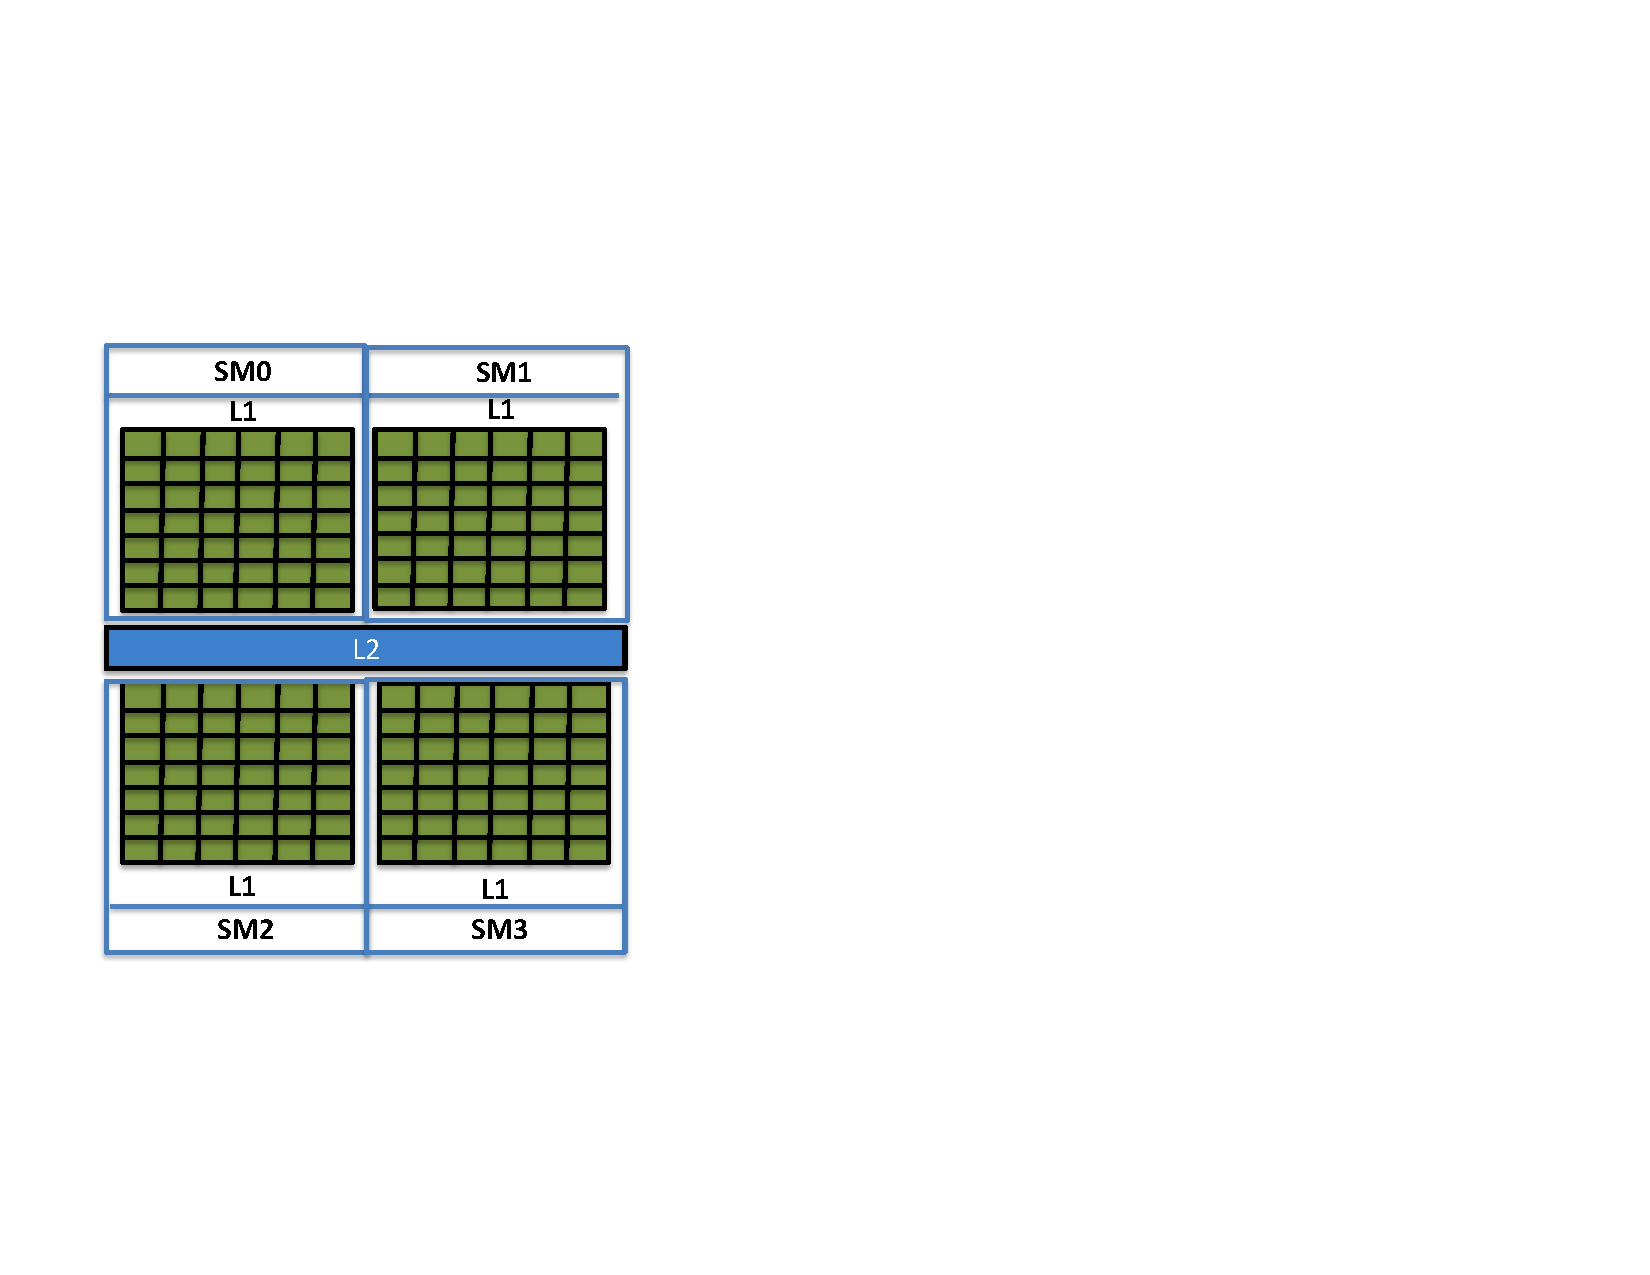
\includegraphics[width=\textwidth]{figures/SMs.pdf}
%\caption{A GPUs with 4 SMs}
%\label{SMs}
%\end{subfigure}
%\begin{subfigure}[b]{0.2\textwidth}
%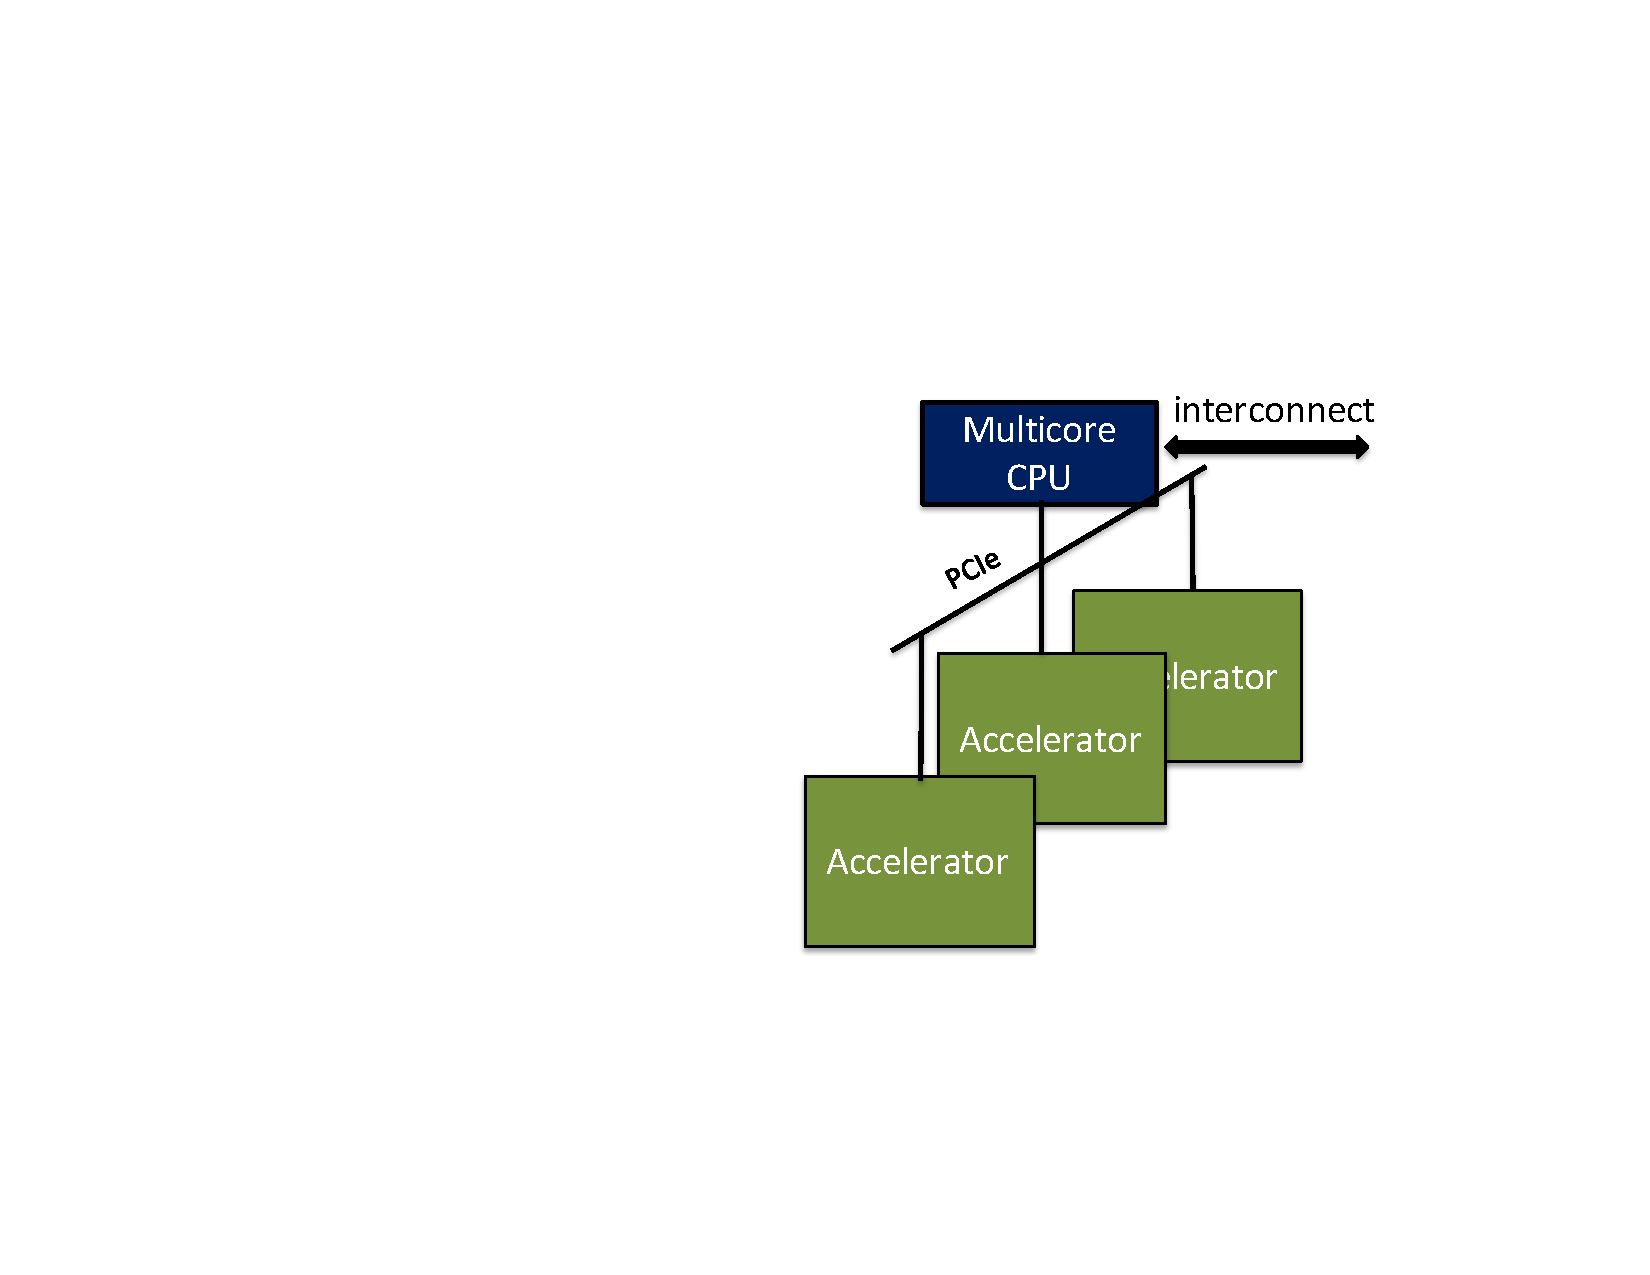
\includegraphics[width=\textwidth]{figures/host_accelerator.pdf}
%\caption{Host with accelerators}
%\label{hybrid}
%\end{subfigure}
%\caption{A hybrid node design}
%\label{fig:sysArch}
%\end{figure}




\section{Programming Model}
\label{sec:model}
In this section, we present the RambutanAcc's task dependency graph programming model and its associated execution model.
Our design goal is to keep the programming API as simple as possible.


\subsection{Task and Data Spaces}
Each RambutanAcc application works on a directed acyclic graph (DAG) in which vertices are {\em tasks} (see Fig.~\ref{fig:cholesky}),
and edges are data or control {\em dependencies}.
{\em RambutanAcc} defines {\em task spaces} and {\em data spaces}.
A task space encapsulates the behavior of a class of tasks.
A task is an atomic sequence of statements, in the sense that when a task is scheduled it runs to completion.
Tasks are created and destroyed dynamically at runtime, so only the active portion of the task graph must reside in memory.
A data space encapsulates access and management of a class of data.
%\cyC{Prefer not to use the term "data partition"}
% The programmer specifies task inputs and outputs, which are data partitions.
The programmer specifies task inputs and outputs, which are called data {\em parcels}.
Each parcel is associated with an attribute called a {\em locale}, which indicates the location of the parcel (e.g. in GPU's memory).
% The programmer defines an ownership function to map tasks to partitions of the data space.
The programmer also defines an ownership function to map tasks to locales.
If a parcel a task requires does not reside in the same locale, the runtime will automatically transfer it.
We next describe the full process of defining a task.

\begin{figure}[htb]
\centering
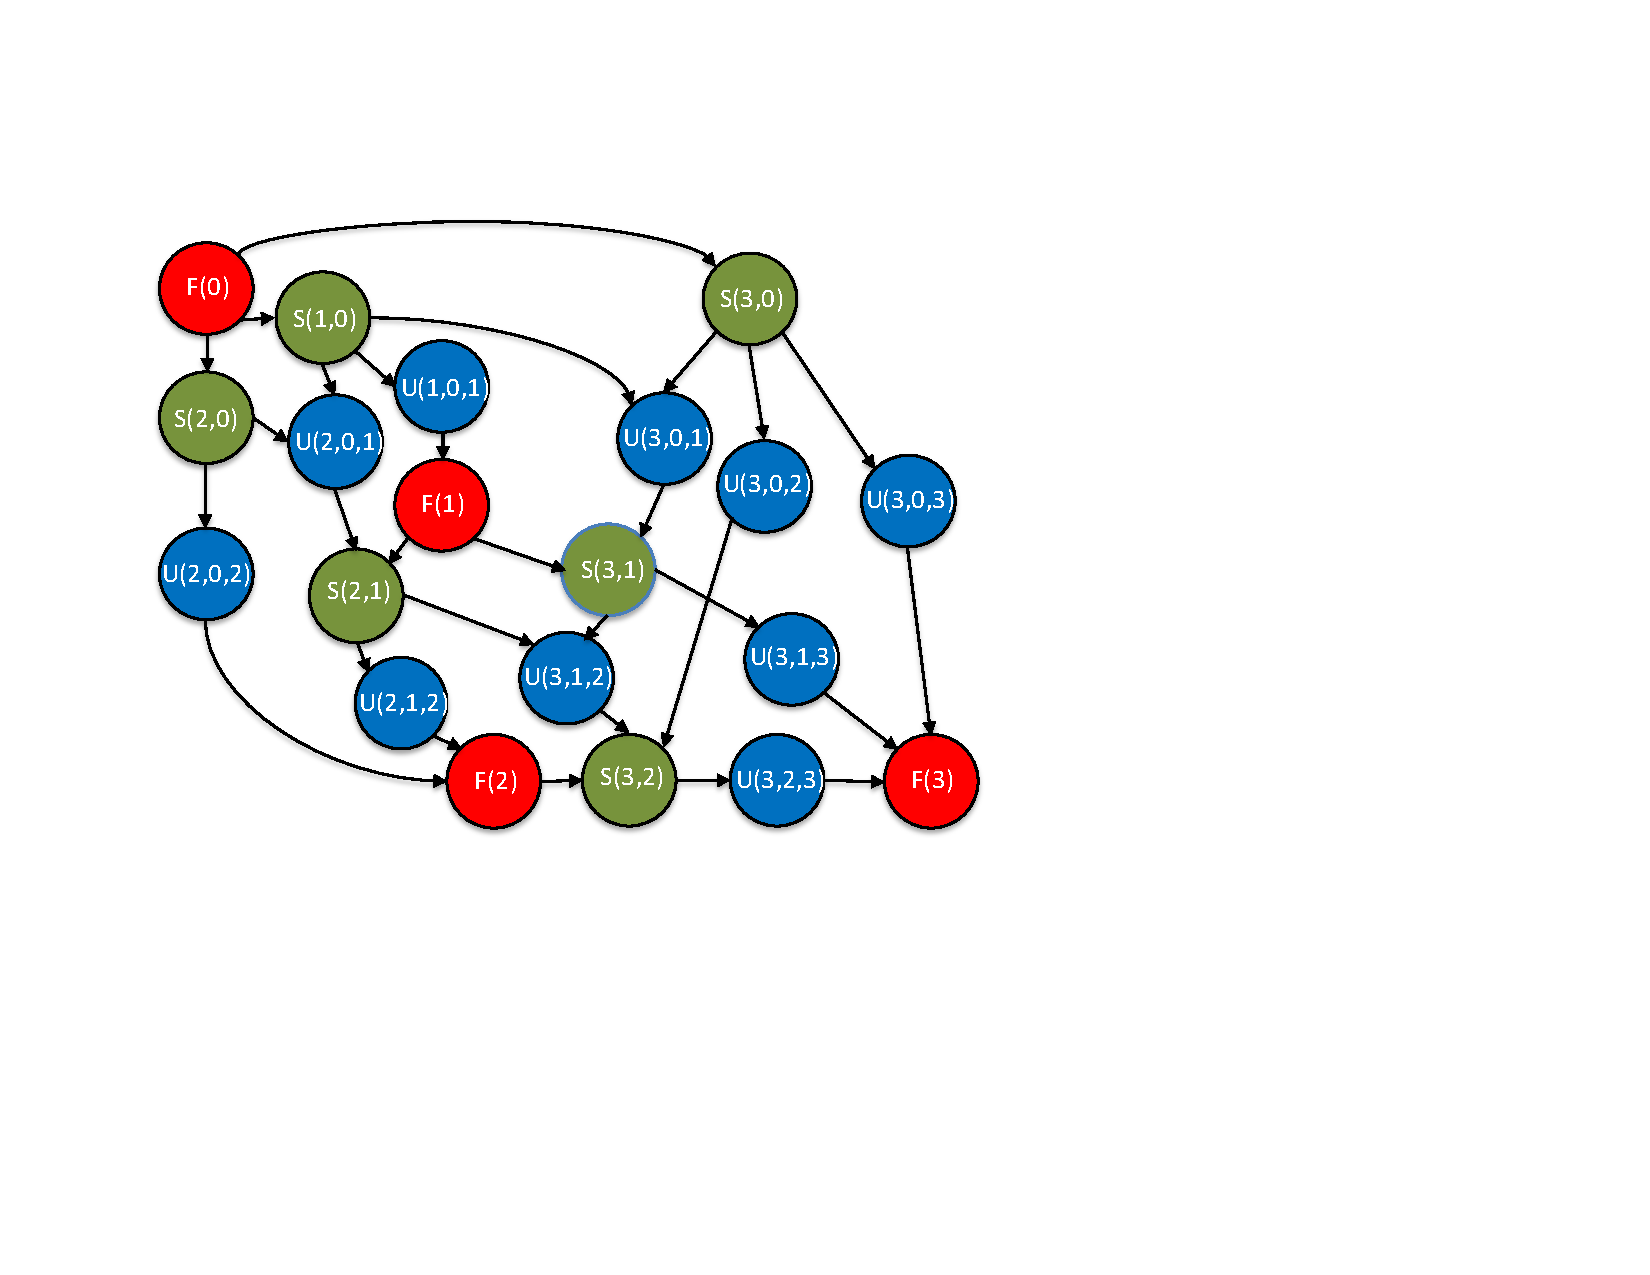
\includegraphics[width=.4\textwidth]{figures/cholesky.pdf}
\caption{Cholesky factorization DAG consisting of three types of tasks: F (Factor), S (Solve), U (update). Each task is associated with a partition of the input matrix called a {\em tile}. Arrows presesent data dependencies between tasks of different types or of the same task type but on different tiles. All data dependencies are called parcels.}
\label{fig:cholesky}
\end{figure}



\subsection{Defining a task}
\label{sec:task-def}
RambutanAcc supports 3 types of task: (1) tasks running completely on the host, (2) tasks running on a group of accelerator cores, and (3) tasks running on host and offload kernels to the accelerator that comes along with host.
The first type supports computation on conventional processors (e.g. Intel's Ivy Bridge, AMD's Opteron, IBM's Power 8)  and many-core processor such as Intel's KNL.
The second type is for studying the benefit of fine-grained scheduling on a group of accelerator cores such as GPU's SM (Symmetric Multiprocessor), whereas the third type is useful when the programmer needs to retain legacy kernel code and study the communication among accelerators.
In the Cholesky factorization graph in Fig.~\ref{fig:cholesky}, it is reasonable to define {\em Factor} and {\em Solve} with the first type since they have low compute intensity. 
{\em Update}, on the contrary, should be defined to run on a group of accelerator cores (type 2) or on the whole accelerator (type 3).

For tasks running completely on the host (type 1), the process of defining a task includes the specification of data inputs and outputs, statements that the task will execute, and actions that should be performed upon completion of the task (e.g. create new tasks).
Defining inputs, outputs, and the post-completion action for tasks of type 2 and 3 are similar to type 1; however, the execution code for these two types is slightly different.
Specifically, the task code must be multithreaded and the abstract thread hierarchy for these tasks is very deep to support a substantially larger number of cores.
Fig.~\ref{fig:program} shows the kernel code of the {\em Update} task of sparse Cholesky factorization, which is a sparse-sparse matrix multiply operation.
Like the CUDA programming model, each task kernel is executed by many threads (called a thread grid), organized into SIMD teams, each scheduled to run on a group of cores.
Teams scheduled (normally in a pipelined fashion) on the same group of cores are called thread blocks.
Type 3 tasks will invoke this kernel using a kernel launch interface (defined by hardware vendor such as NVIDIA) with many threads occupying the whole accelerator and hiding the latency from DRAM to registers.
For performance advantage, we expect the kernel launch to be asynchronous (though synchronous is fine for correctness).
The asynchronous launch returns a handle (e.g. a CUDA stream handle) and RambutanAcc only executes the post-completion action once this handle indicates that the kernel code on the accelerator has completed.
Unlike type 3, type 2 tasks do not have to spawn threads to occupy the whole accelerator.
RambutanAcc pre-spawns persistent kernels, and we utilize more threads than cores to hide the DRAM latency.
The task code is automatically offloaded to the accelerator by RambutanAcc's task scheduler.
No handle is needed in this case since RambutanAcc offloads the code and it is aware of when the code finishes.


\begin{figure}[htp]
\lstinputlisting[caption=]{code/example.c}
\caption{Kernel code of a task is executed by teams of threads. Each team is mapped to a group of accelerator cores and threads within the team are mapped to cores in the group. Teams mapped to the same group are called block. Note that for GPUs, each team should be a multiple of 16 SIMD threads to avoid thread divergence.}
\label{fig:program}
\end{figure}


\subsection{Execution model}
We next explain how the entire task dependency graph executes.
At the highest level, the graph is serviced by one or more processes, each consisting of one or more {\em workers}.
As previously mentioned, these workers can be CPU cores, accelerators, or groups of accelerator cores.
At the beginning, tasks that can run without any input dependencies are called {\em roots} of the graph, and they can be scheduled immediately.
In the task graph program described in Fig.~\ref{fig:cholesky}, task {\em F(0)} is the only root.
Once a root task finishes its execution, output data parcels may be produced.
Through the post-completion action, the task notifies the runtime about the availability of the data parcels so the runtime can create new tasks and transfer the parcels to where they are needed.
Note that the programmer has flexibility to control the location of newly created tasks, so task creation on a remote process is allowed.
As soon as the data required by a task has been fetched by the runtime, that task becomes runnable
and will be scheduled to execute on a worker.
The runtime scheduler periodically checks the availability of workers to schedule tasks.
A worker can be configured with a private task queue so that the scheduler can assign it new tasks even when the worker is already executing.
This capability allows tasks to be offloaded to workers on the accelerator at zero cost, since the time to move required data from host to accelerator can be overlapped with the execution of other tasks.

%A notable concern when programming on accelerators is that the DRAM capacity on accelerator is often modest compared to host DRAM.
%If this is the case, the programmer often decides to keep data on the host and stream only a portion of data to the accelerator at a time to compute before streaming the results back.
%Thus, if there are too many tasks created at the same location resulting in so much data being simultaneously fetched to that location, one may run out of memory.
%Since {\em RambutanAcc} allocates temporary buffers to perform the fetching work, it has the ability to maintain a reasonable amount of buffer to avoid this problem.


%\subsection{Example}
%Fig.~\ref{fig:firstProgram} presents some pseudo code to illustrate how a task can be defined to execute on the GPUs.
%Lines \#11 to \#17 show how a task registers with the runtime about inputs and outputs.
%In this case, a task depends on {\tt Unew} of the previous iteration and ghost cells of other tasks.
%The {\em dataMapping} function should swap {\tt Unew} and {\tt Old} for every iteration.
%All these data arrays reside in GPU DRAM.
%The {\em execute()} function offloads the function that will be executed and required arguments.
%System arguments such as thread and block indices are given by the runtime.




\section{Implementation}
\label{sec:impl}
In this section we present the implementation details of {\em RambutanAcc}.
At the high level, the runtime is constituted of three major modules: task management system, communication handler, and task scheduler as shown in Fig.~\ref{fig:impl}. 
The runtime can be configured to run on a dedicated processor core in order to keep it responsive.

\begin{figure}[htb]
\centering
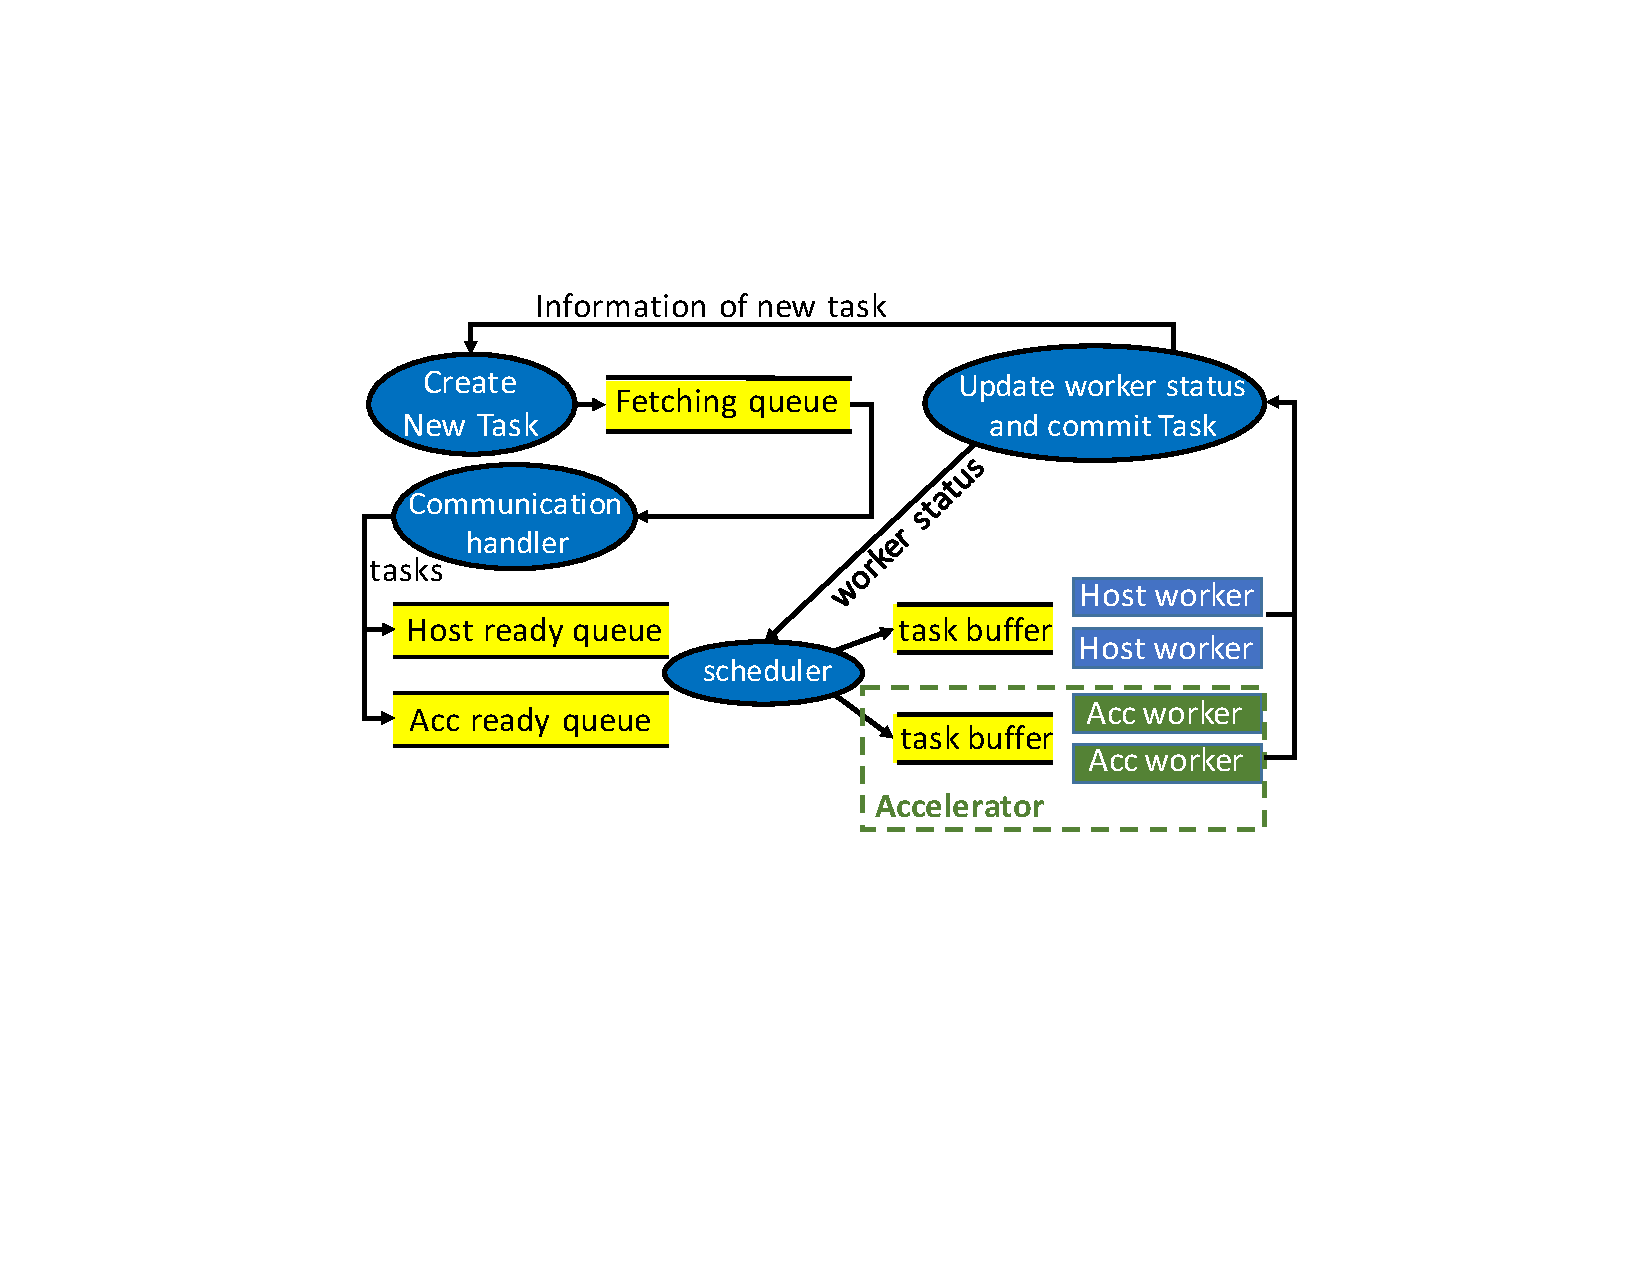
\includegraphics[width=.49\textwidth]{figures/impl.pdf}
\caption{Runtime implementation}
\label{fig:impl}
\end{figure}

\subsection{Task Management System}
Tasks can be created as soon as input data are produced.
The task management system listens for requests from existing tasks to create new tasks.
A task may own data.
Upon the completion of a task, the task management system may write data back (if necessary) before destroying the task.
If the task executed on accelerator while original data resides in host memory, data will be written back to host asynchronously, overlapping with other tasks' computations.
If original data locate in a different place, the task management system asks the communication handlers to write data back.

\subsection{Communication handlers}
Once a task has been created, it will be pushed to the {\em fetching queue} by the task management system.
The communication handler periodically pulls tasks from this queue and fetches their input data.
Depending on the available memory resource, a certain number of tasks in the {\em fetching queue} will be served at a time.
{\em RambutanAcc} supports both on-node and off-node communication.

Within a single node, we use communication primitives provided by the accelerator's vendor.
In particular, on compute nodes with NVIDIA GPUs, we use CUDA stream to move data between host and GPUs.
On Intel's KNC-based nodes, we use COI (Coprocessor Offload Infrastructure)\samW{citation for COI??}.
To avoid blocking the runtime, we don't use any synchronization routine.
Instead, the communication handler periodically tests the completion of communication activities.

We employ GASNet to implement the off-node communication handler.
The process of fetching data from a remote node is shown in Fig.~\ref{fig:offnode}.
To fetch remote data for a task, the corresponding GASNet process issues a remote procedural call to request data from the process that holds the task owning the data (1).
This procedure looks for the appropriate data at the remote node.
If the data resides in accelerator memory, the remote procedure has also to pull the data up before sending the data (2).
Once the memory transfer from accelerator completes (3), the data can be sent to the requester using the one-sided {\em put} operation (4).
Once the remote GASNet process finishes the remote data transfer, it issues a response remote procedural call to push the data to the accelerator of the requester (if necessary) and notify the requester when data is available for the task.
All these activities run asynchronously, and we use a polling mechanism to avoid blocking the runtime.
The process of writing data back is similar to the fetching process, and it is also handled asynchronously.


\begin{figure}[htb]
\centering
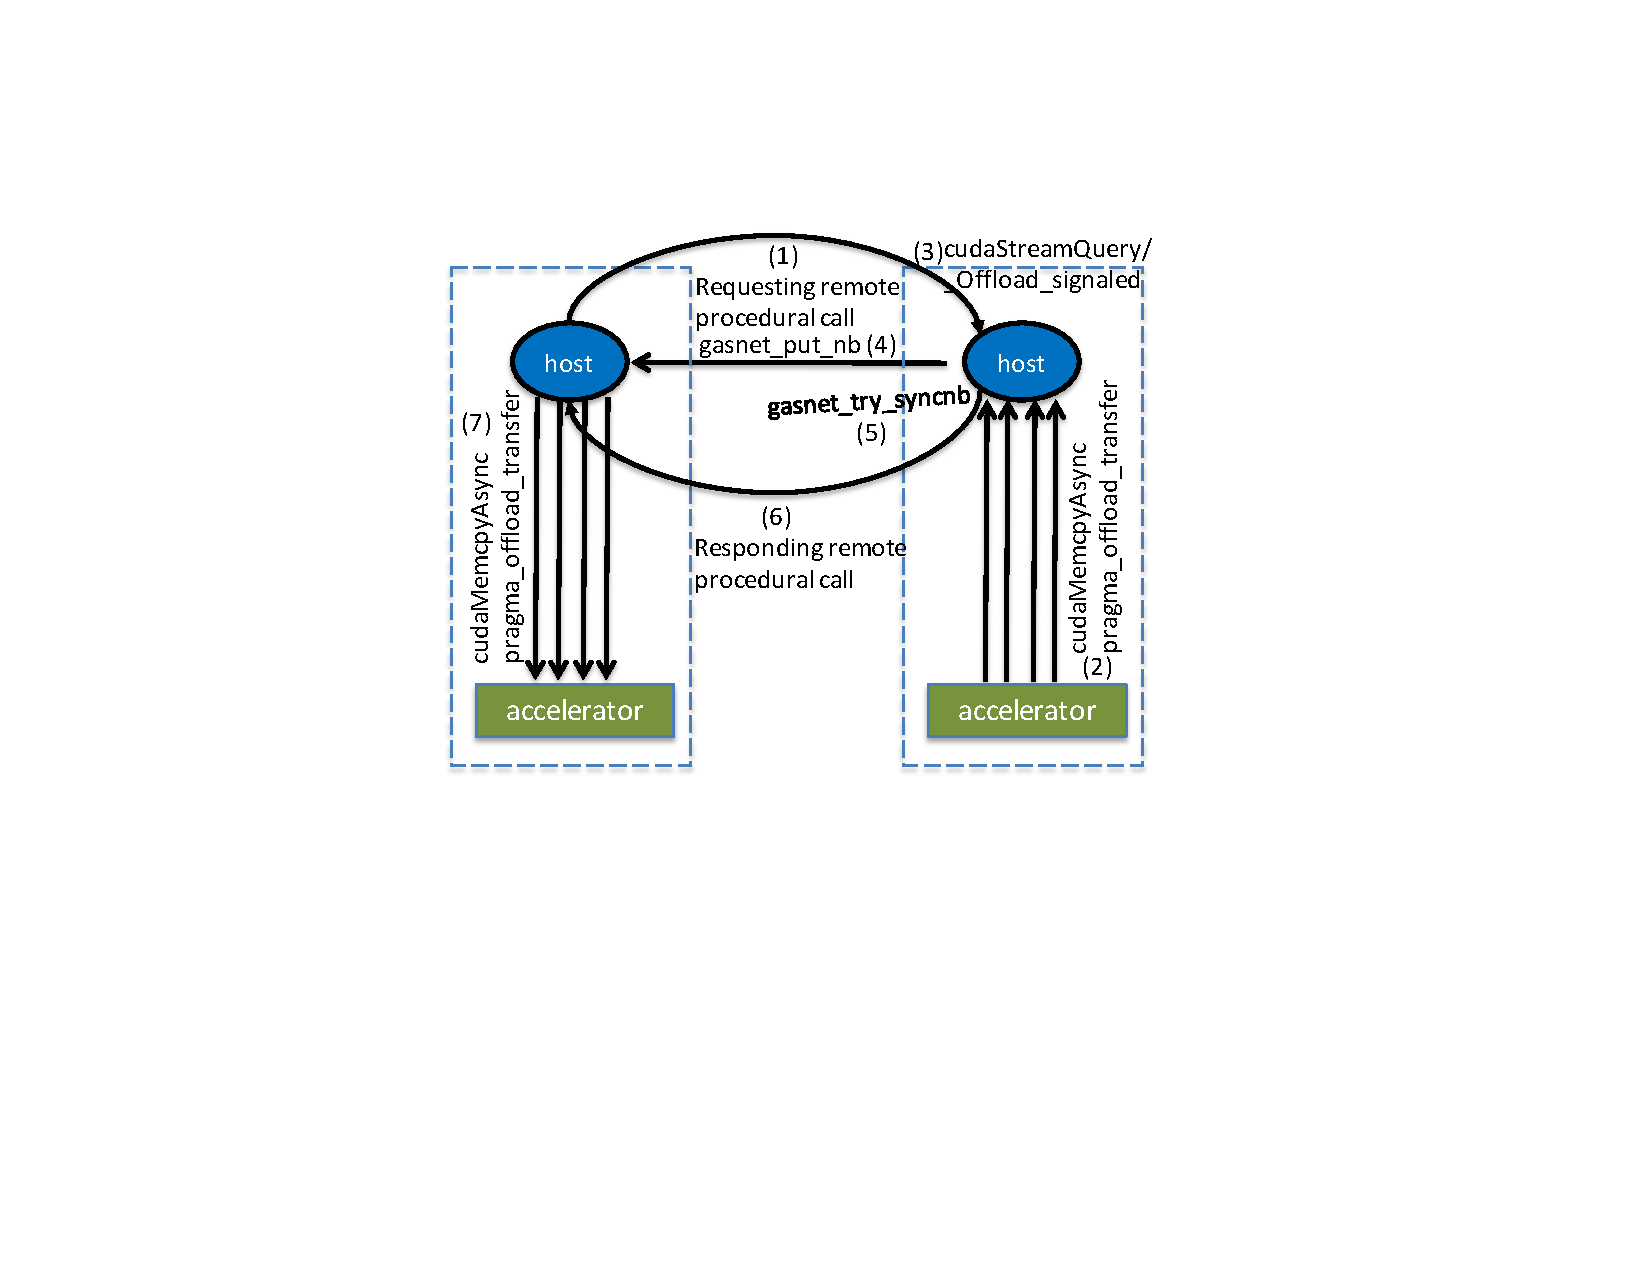
\includegraphics[width=.49\textwidth]{figures/handler.pdf}
\caption{Implementation of the off-node communication handler}
\label{fig:offnode}
\end{figure}

\subsection{Task Scheduler}
Tasks become {\em ready} and pushed in the {\em ready queues} once all of their data have been fetched.
Each GASNet process runs a task scheduler to dispatch {\em ready tasks} to workers. 

\subsubsection{Task Buffer}
To keep workers busy, the scheduler frequently checks the runnable task queue and the status of workers.
However, the task scheduler may not be very responsive since the communication handlers also run on the same processor core.
Thus, each worker has a task buffer with a few slots.
The scheduler fills up these slots while the workers keep popping tasks and executing.
To reduce synchronization overheads we use a lock-free implementation for this single producer-multiple consumers scheme.

\subsubsection{Acc worker using CUDA persistent kernel}
Since the host worker implementation is simple, we now present the implementation of accelerator workers on GPUs.
A {\em RambutanAcc} program just launches a CUDA kernel to set up workers on the GPUs' SMs and execute assigned tasks.
Once the kernel is launched, CUDA thread blocks find out what SM they are mapped to by the CUDA runtime.
Accessing this information is possible by inserting PTX code to read a special register that holds the SM ID.
As shown in Fig.~\ref{fig:kernel}, we keep only a certain number of thread blocks per SM (this number can be set via an environment variable and the default value is 1).
The reason is that thread blocks run until the program completes and the CUDA runtime co-runs only a limited number of thread blocks on the same SM.
The alive thread blocks will be divided into workers.
Each worker is a group of thread blocks, acting as the new CUDA grid for scheduled tasks.

\begin{figure}[htb]
\centering
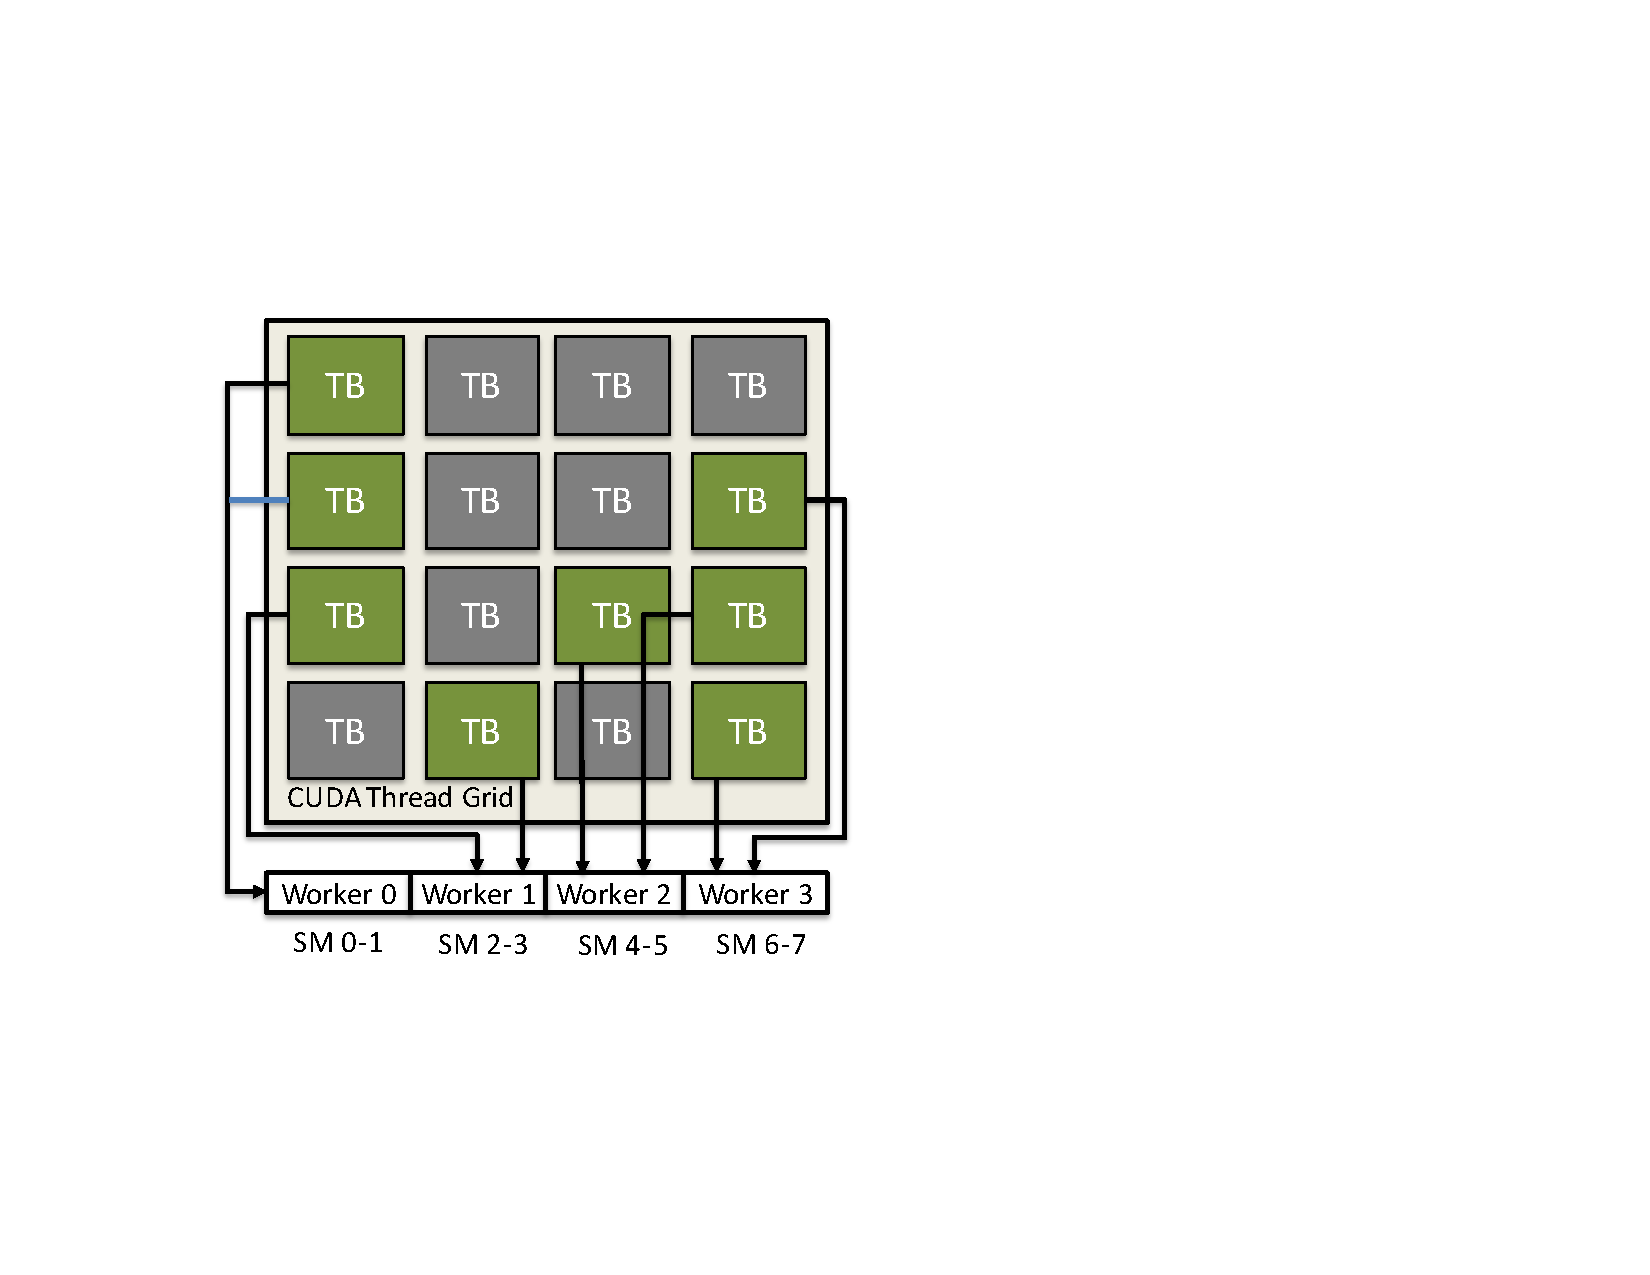
\includegraphics[width=.35\textwidth]{figures/kernel_init.pdf}
\caption{The persistent kernel selects only a limited number of thread blocks per SM (green color). The default number of thread blocks per SM is 1. 
The alive thread blocks are divided into workers to execute tasks.}
\label{fig:kernel}
\end{figure}

Now each thread block knows which worker it belongs to and where to find tasks to execute.
Once there are ready tasks and an available worker slot, the scheduler offloads corresponding function and arguments to task buffers on the GPUs.
Then the scheduler picks a worker and notifies it by writing a signal to the GPU using the nonblocking copy {\em cudaMemcpyCpyAsync}.
If the worker is busy at the time, it will read the signal  and execute the corresponding task later.
Once the task finishes, the worker notifies the scheduler.
Since a CUDA kernel cannot send data to the host, we have to use UVM (unified virtual memory).




\section{Experimental Results}
\label{sec:results}
\subsection{Experimental Testbed}
In this section, we employ RambutanAcc to study the impact of various code optimizations at different hardware levels of a GPU cluster.
Since an application generally benefits from only a subset of these optimizations, we need more than one application.
To this end, we take four benchmarks commonly used in science and engineering: sparse cholesky factorization, a machine learning based face recognition code, 2.5D Cannon's Matrix Multiplication, and a 3D Stencil.
When studying optimizations on a single GPU, to have apples-to-apples comparisons we always use our own CUDA kernels instead of 3rd party implementations (e.g. cuSPARSE). 
In particular, for Sparse Cholesky Factorization, we develop our own CUDA kernels for $C = \alpha* A * B + \beta C$ where either A, B, and C are all in the {\em sparse} form or A is dense and B and C are sparse.
In these kernels, we perform many optimization techniques such as memory coalescing and spatial tiling.
We also employ a warp based thread reduction implementation that minimizes memory accesses. 
For studies at higher hardware levels, we use vendor provided kernels as much as possible.
For example, in  2.5D Cannon we use the cuBLAS's {\em dgemm} and {\em daxpy} implementations included in the NVIDIA toolkit to perform local matrix multiplication.

For node level optimizations (on single and multiple GPUs of the same compute node), we use up to three K80 GPUs.
A K80 GPU pairs two GPU cards each having 2496 CUDA cores organized into 13 SMs.
The whole K80-based system is equipped with 24GB DRAM with up to 480 GB/s memory bandwidth.
For cluster level optimizations, we run code on K20 GPUs on Titan.
We use the nvcc compiler version 7.0 and sm\_35 capability for CUDA codes and the Intel compiler for codes running on the host.
We use GASNet for communication among GPUs. 


\subsection{Scheduling tasks on SMs of a GPU}

\subsubsection{Sparse Cholesky Factorization}
Sparse Cholesky Factorization A= $LL^T$, where A is a sparse and symmetric positive-definite matrix,
appears in many scientific and engineering problems.
Depending on the sparsity pattern of the input matrix, many sparse representations can be used.
In this paper we employ the CSC (Compressed Sparse Column) format. 
The input matrix is organized as a list of "non-zero" tiles, each including lists of non-zero elements and their row and column indices.
The factorization operation is comprised of three smaller kernels: {\em factor}, {\em solve}, and {\em update}.
These computations on CSC tiles and their data dependencies can be represented by a DAG as shown in Fig.~\ref{fig:cholesky}. 
For very sparse matrices, this DAG may consist of many small tasks.
Thus, this is a perfect application to evaluate the benefit of the fine-grained task scheduling support of the runtime.
We place data on the host's DRAM and execute {\em factor} and {\em solve} on the host's worker.
The compute-intensive {\em update} kernel is executed on the GPU workers.
{\em RambutanAcc} automatically streams data required by this kernel to the GPU's DRAM and streams the results back.

\begin{figure}[htb]
\centering
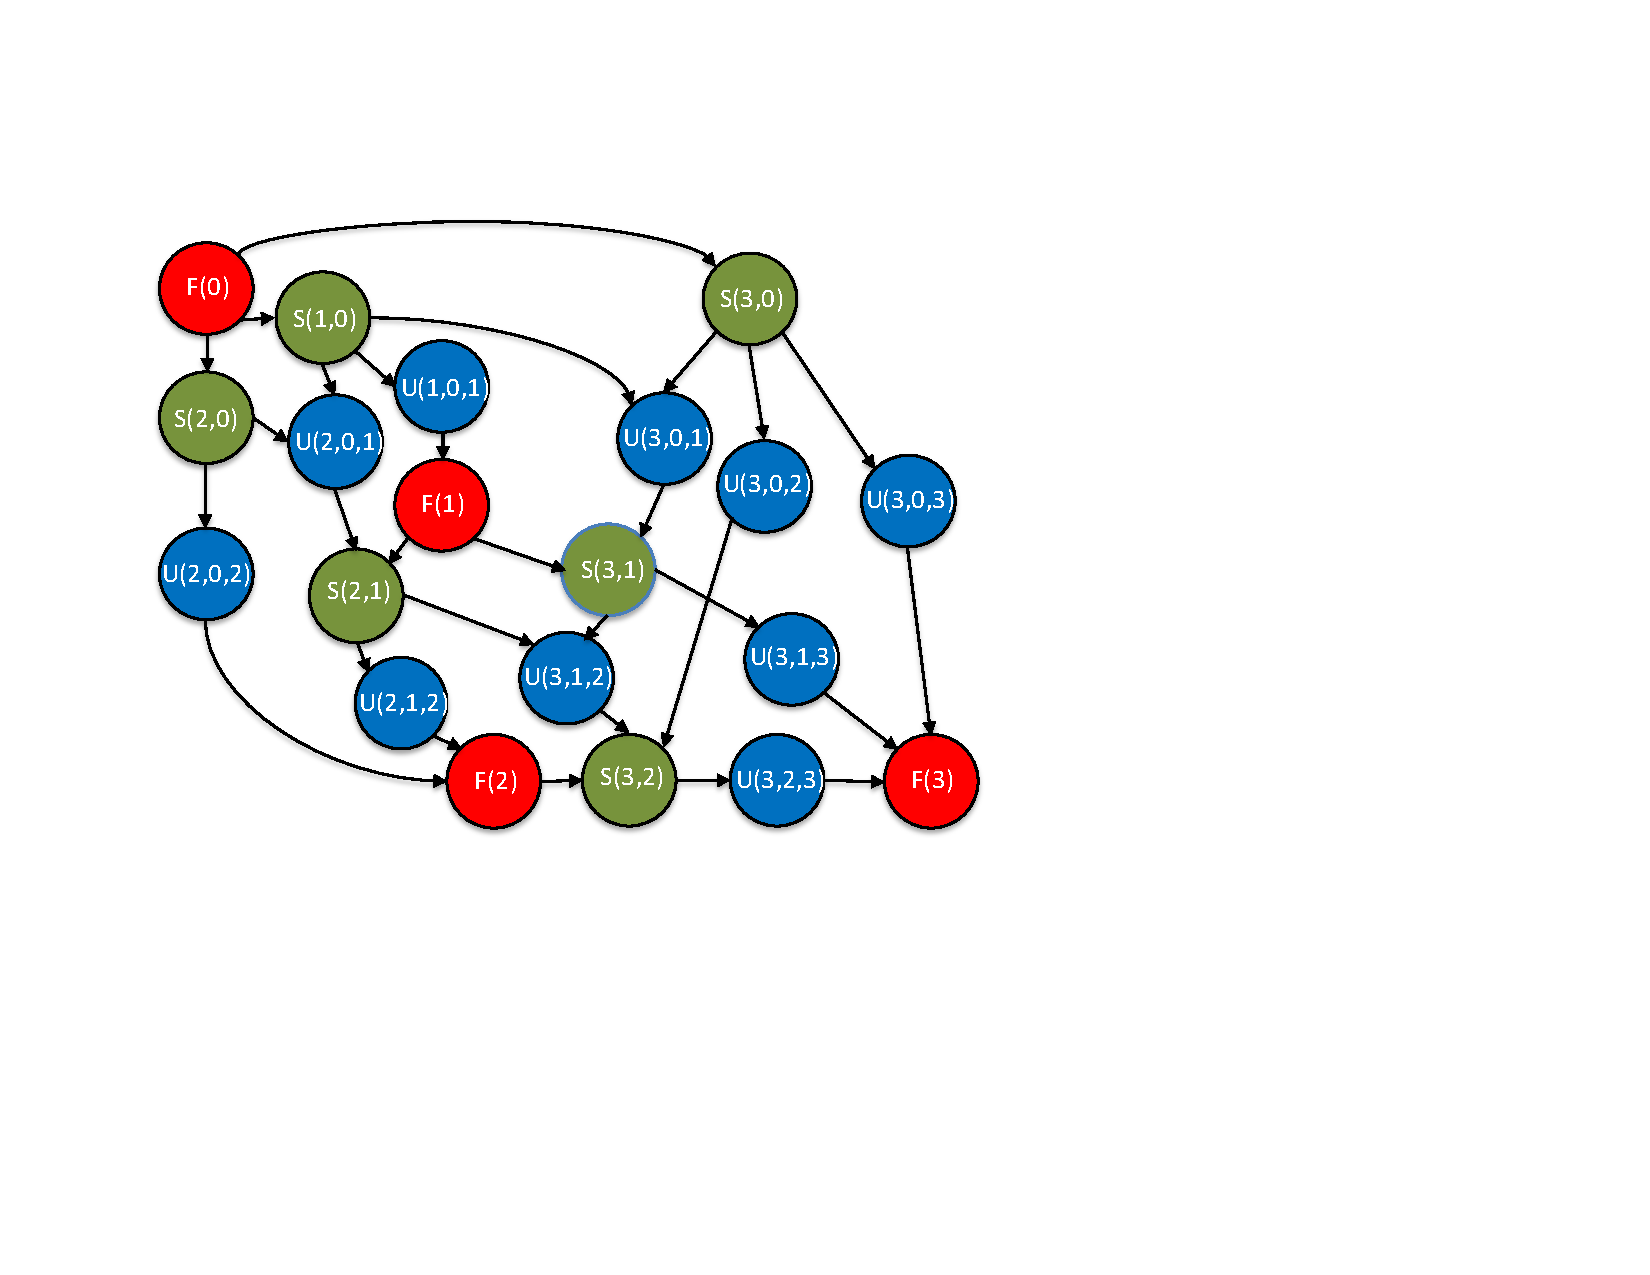
\includegraphics[width=.3\textwidth]{figures/cholesky.pdf}
\caption{Cholesky factorization DAG consisting of three types of tasks: F (Factor), S (Solve), U (update). Each task is associated with a partition of the input matrix called a {\em tile}. Arrows presesent data dependencies between tasks of different types or of the same task type but on different tiles.}
\label{fig:cholesky}
\end{figure}


An interesting path to explore is the tradeoff between coarse and fine-grained scheduling policies.  
For sparse cholesky, the matrix is represented by many small CSC tiles.
Thus, even a small problem size can result in many tasks.
Fig.~\ref{fig:coarseFine} shows results of sparse cholesky under two scheduling policies.
It can be seen that fine-grained scheduling policy outperforms the coarse-grained one.
This can be explained as follows.
Each CSC tile is very small (e.g. 32$\times$32), making it hard to map computations efficiently to many CUDA cores.
Thus, it may not be posible to scale a task to all available SMs of a GPUs.
We observe that for many input matrices tasks run more efficiently after reducing the number of SMs per worker by a factor of 2$\times$ or 4$\times$.
Since there are many tasks that can be runnable at a time, the scheduler can keep all SMs busy at very small overhead.
Fig~\ref{fig:nWorkers} shows the optimal number of workers on a K80 GPU for Sparse Cholesky Factorization when the degree of sparsity of the input matrix varies.
If the sparse matrix is filled with many tasks we have more parallelism, allowing us to configure the GPUs with more workers.

The lesson learn from this study is that fine-grained scheduling can be very helpful if we have a DAG with many small tasks, which can not run well on the whole GPU-based system.
This is an important observation since sparse representation is very common in practice.
{\em RambutanAcc} runtime supports fine-grained task scheduling, a simple yet powerful solution to this problem.
The programmer can obtain high compute throughput on GPUs without complicating the application algorithm.

\begin{figure}[htb]
\centering
\begin{subfigure}{0.23\textwidth}
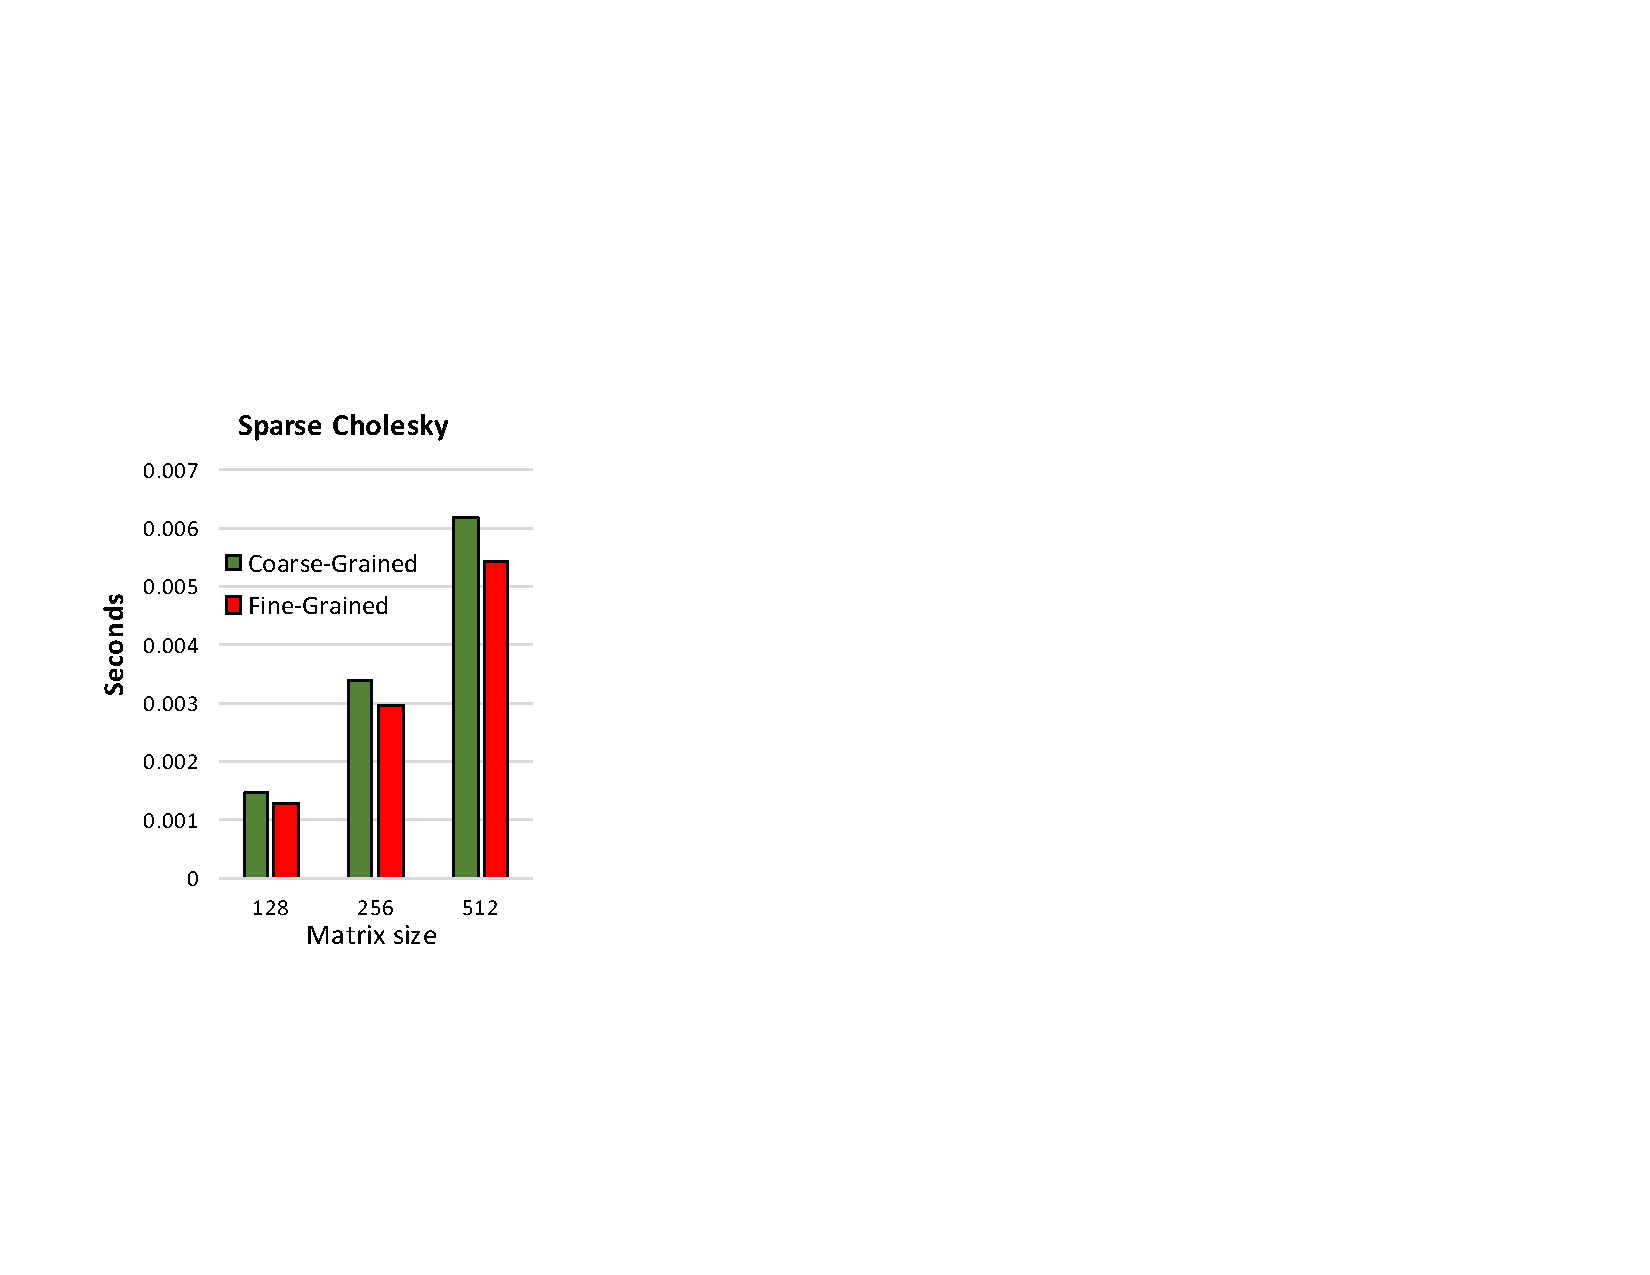
\includegraphics[width=\textwidth]{figures/choleskyScheResults.pdf}
\caption{Tile size 32$\times$32}
\label{choleskySche}
\end{subfigure}
\begin{subfigure}{0.23\textwidth}
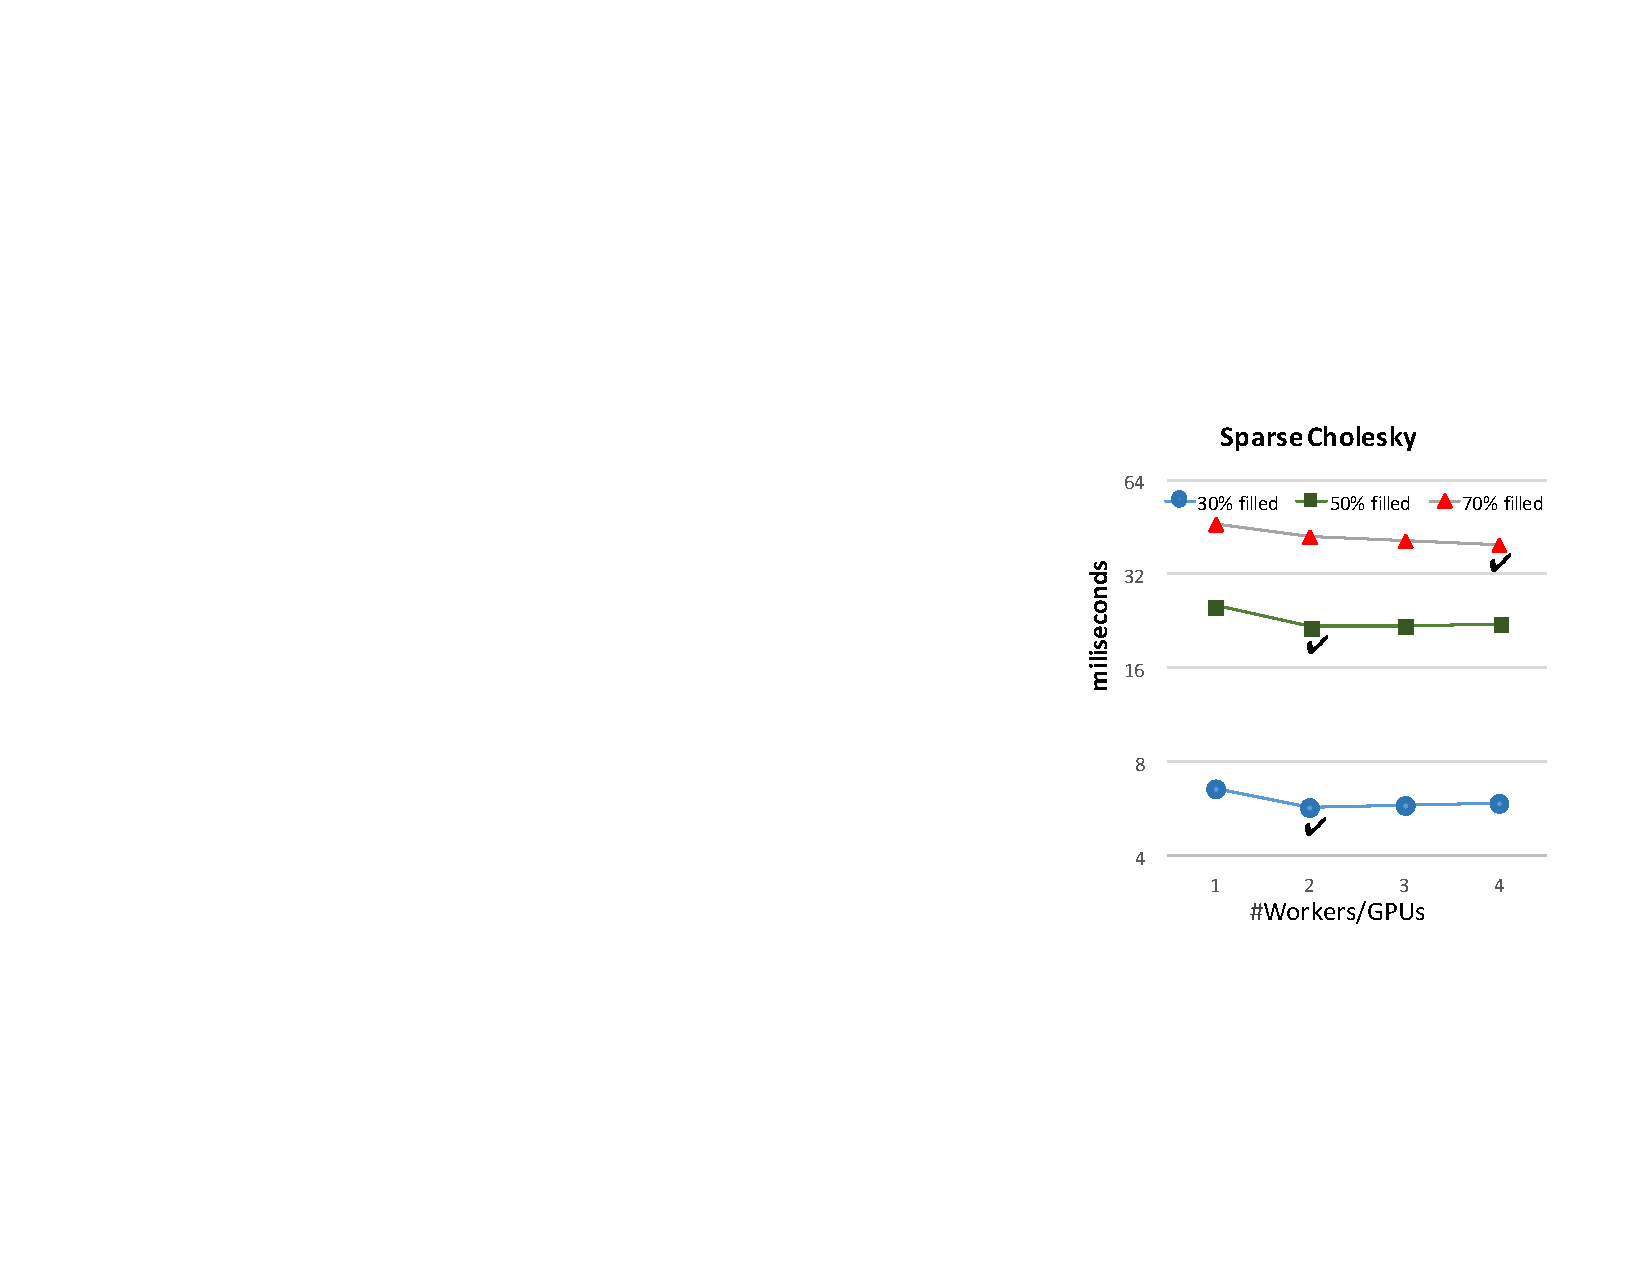
\includegraphics[width=\textwidth]{figures/nWorkers.pdf}
\caption{The optimal number of workers/GPUs}
\label{fig:nWorkers}
\end{subfigure}
\caption{Coarse v.s. fine-grained Scheduling}
\label{fig:coarseFine}
\end{figure}


\subsubsection{Viola-Jones Face Recognition}
We next study the impact of dynamic task scheduling in balancing the workload among SMs of a GPU.
For this study we use the Viola-Jones face detection kernel, an important module in many applications such as security surveillance.
The Viola-Jones face detection algorithm detects faces by scanning a regtangular window of pixels over the image where it looks for features of a human face. 
If a window contains a significant number of these features, it is considered to be a face. 
Since face size varies, the window is scaled a number of times and the scanning process is repeated. 
To reduce the number of features that each window needs to check, the window passes through a number of different stages. 
Early stages have fewer features to check and are easier to pass whereas later stages have more features and are more selective. 
At each stage, the calculations of features are accumulated and, if this accumulated value does not pass the threshold, the stage is failed and the current window is considered to not contain a face. 

For this application, it is straightforward to exploit parallelism among search windows.
Each CUDA thread block is responsible for a fixed number of windows, which will be further distributed to threads within the thread block.
We call this code variant {\em CUDA-Basic}.
Since the number of instructions per window depends on the input, the impact of thread divergion is expected to be significant.
Thus, we also employ a {\em CUDA-Static Warp Scheduling} version which allows 32 threads in a warp to share a window (and thus they perform the same number of instructions).
Porting this code on RambutanAcc, we expect to improve the performance further by balancing the workload among these warps.
Finally, we run a hand-optimized code variant, which embeds the task scheduler into the kernel code.
This code has all the capabilities that RambutanAcc can, but at lower cost since the task scheduler is specialized and runs on the GPU.

\begin{figure}[htb]
\centering
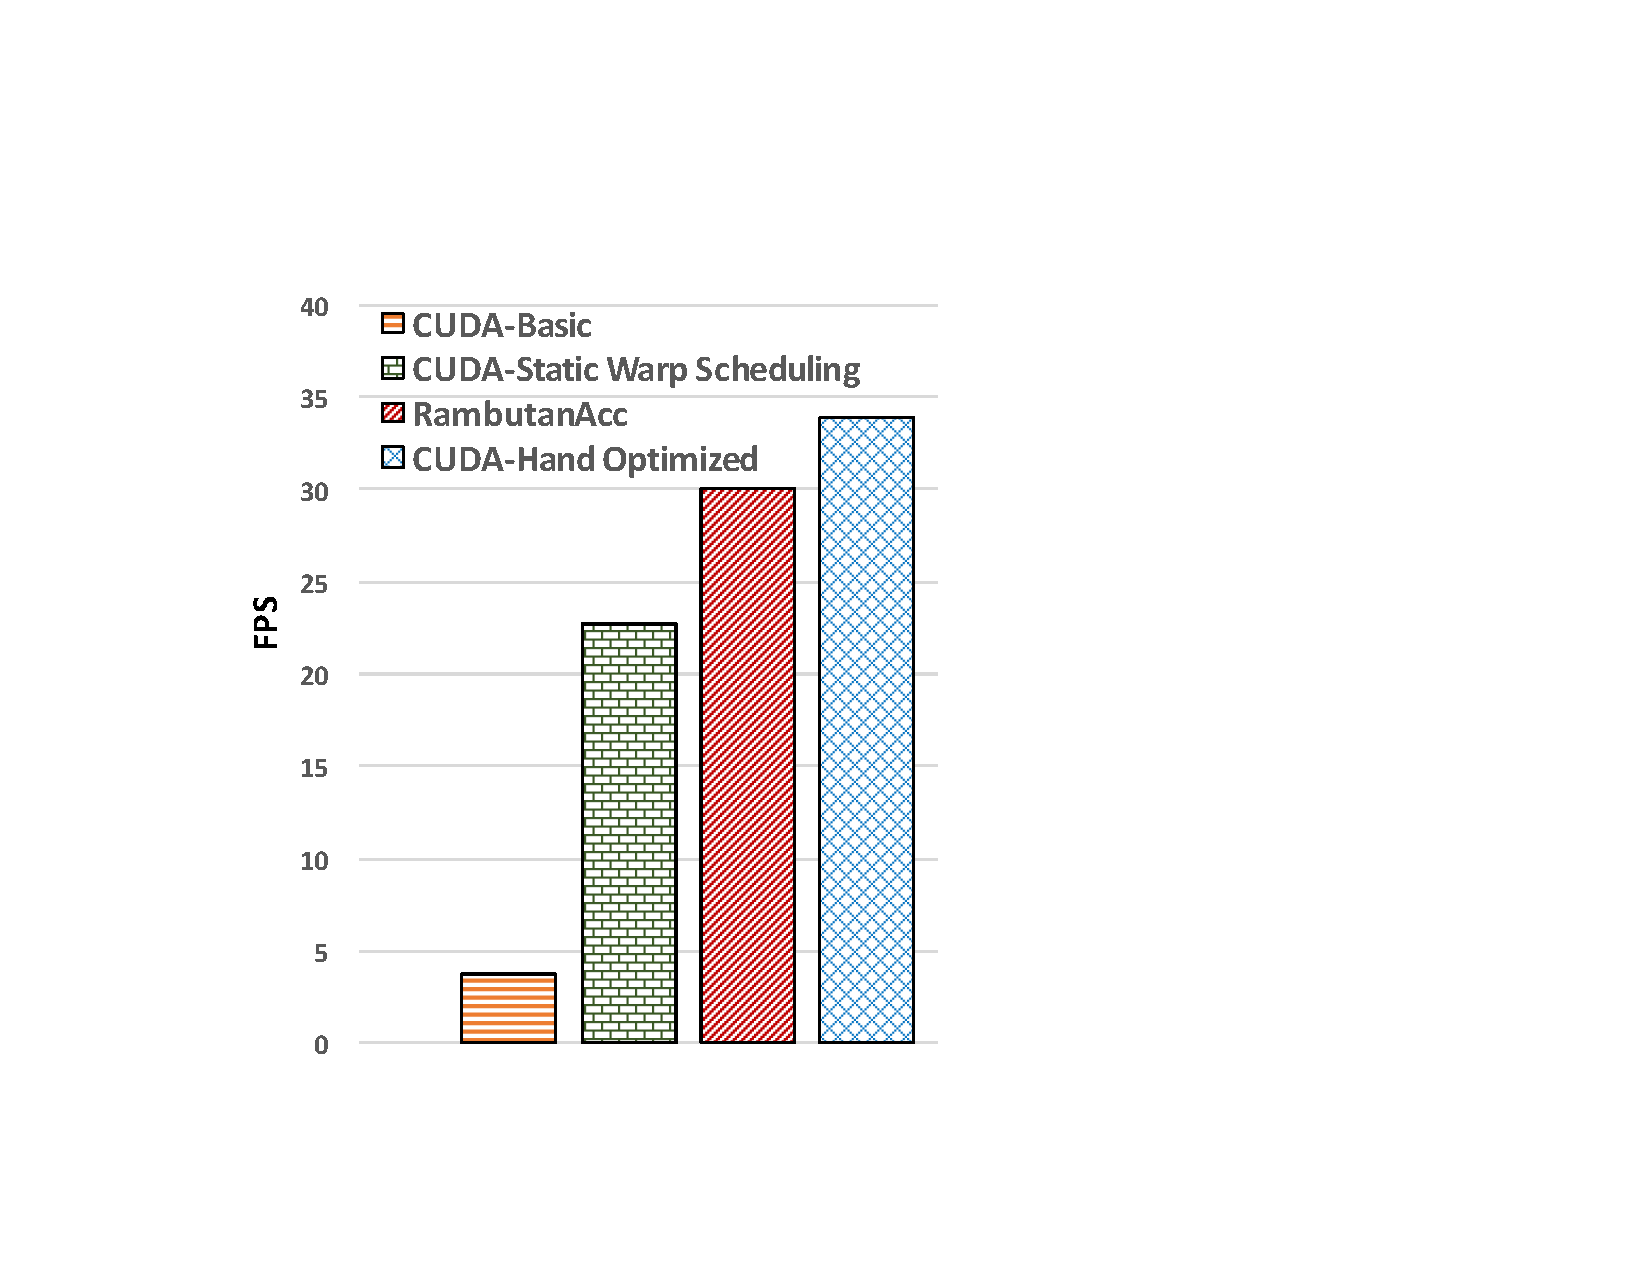
\includegraphics[width=0.35\textwidth]{figures/faceRecognition.pdf}
\caption{Balance the face searching}
\label{faceRecognition}
\end{figure}

Fig.~\ref{faceRecognition} shows the performance of all code variants.
{\em CUDA-Basic} performs poorly as expected.
Under this straightforward strategy, only one or a few threads among 32 threads of the same warp reach to late stages while the rest stay idle.
This explains why {\em CUDA-Static Warp Scheduling} improves the performance significantly.
However, there remains significant load imbalance among warps.
With RambutanAcc, windows are distributed to workers dynamically.
Specifically, we configure the runtime with 26 workers (two workers per SM), each a CUDA thread block. 
The scheduler running on the host keeps assigning blocks of windows to these workers.
In order to hide the scheduling latency, we configure the task buffer of each worker with multiple slots.
While the worker is processing the current window block, the scheduler can offload another block to the remaining slots.
In this experiment, each block takes about 50$\mu$s to finish, whereas the offloading cost is around 10$\mu$s.
Thus, configuring the task buffer with two slots is sufficient.
Fig.~\ref{faceRecognition} shows that RambutanAcc speeds up {\em CUDA-Static Warp Scheduling} by 1.35$\times$.
All the performance improvement can be attributed to the capability of balancing computationgs among SMs of the GPU.
The {\em CUDA-Hand Optimized} version runs even faster.
The additional performance improvement is due to reducing scheduling overhead by embedding the scheduler to the application source code.


\subsection{Scheduling tasks on GPUs of the same node}

\subsubsection{3D Stencil}
On multiple GPUs we pick {\em 3D Stencil}, an iterative solver for Laplace's equation in three dimensions.
{\em 3D Stencil} iterates over a 3D mesh, updating data elements using values from six nearest neighbors.
The DAG for this application is similar to that shown earlier in Fig.~\ref{fig:taskGraph}, except for the number of dimensions.
In particular, each task is associated with a data partition with up to six ghost cells.
A task can be run when the previous iteration on this data partition finishes and it pulls all the needed ghost cells from neighboring tasks.
3D stencil is a memory bandwidth bound application. 
Thus using GPUs can boost up the performance significantly.
It is interesting to determine if {\em RambutanAcc} can improve the performance further by  hiding communication overheads.

\begin{figure}[htb]
\centering
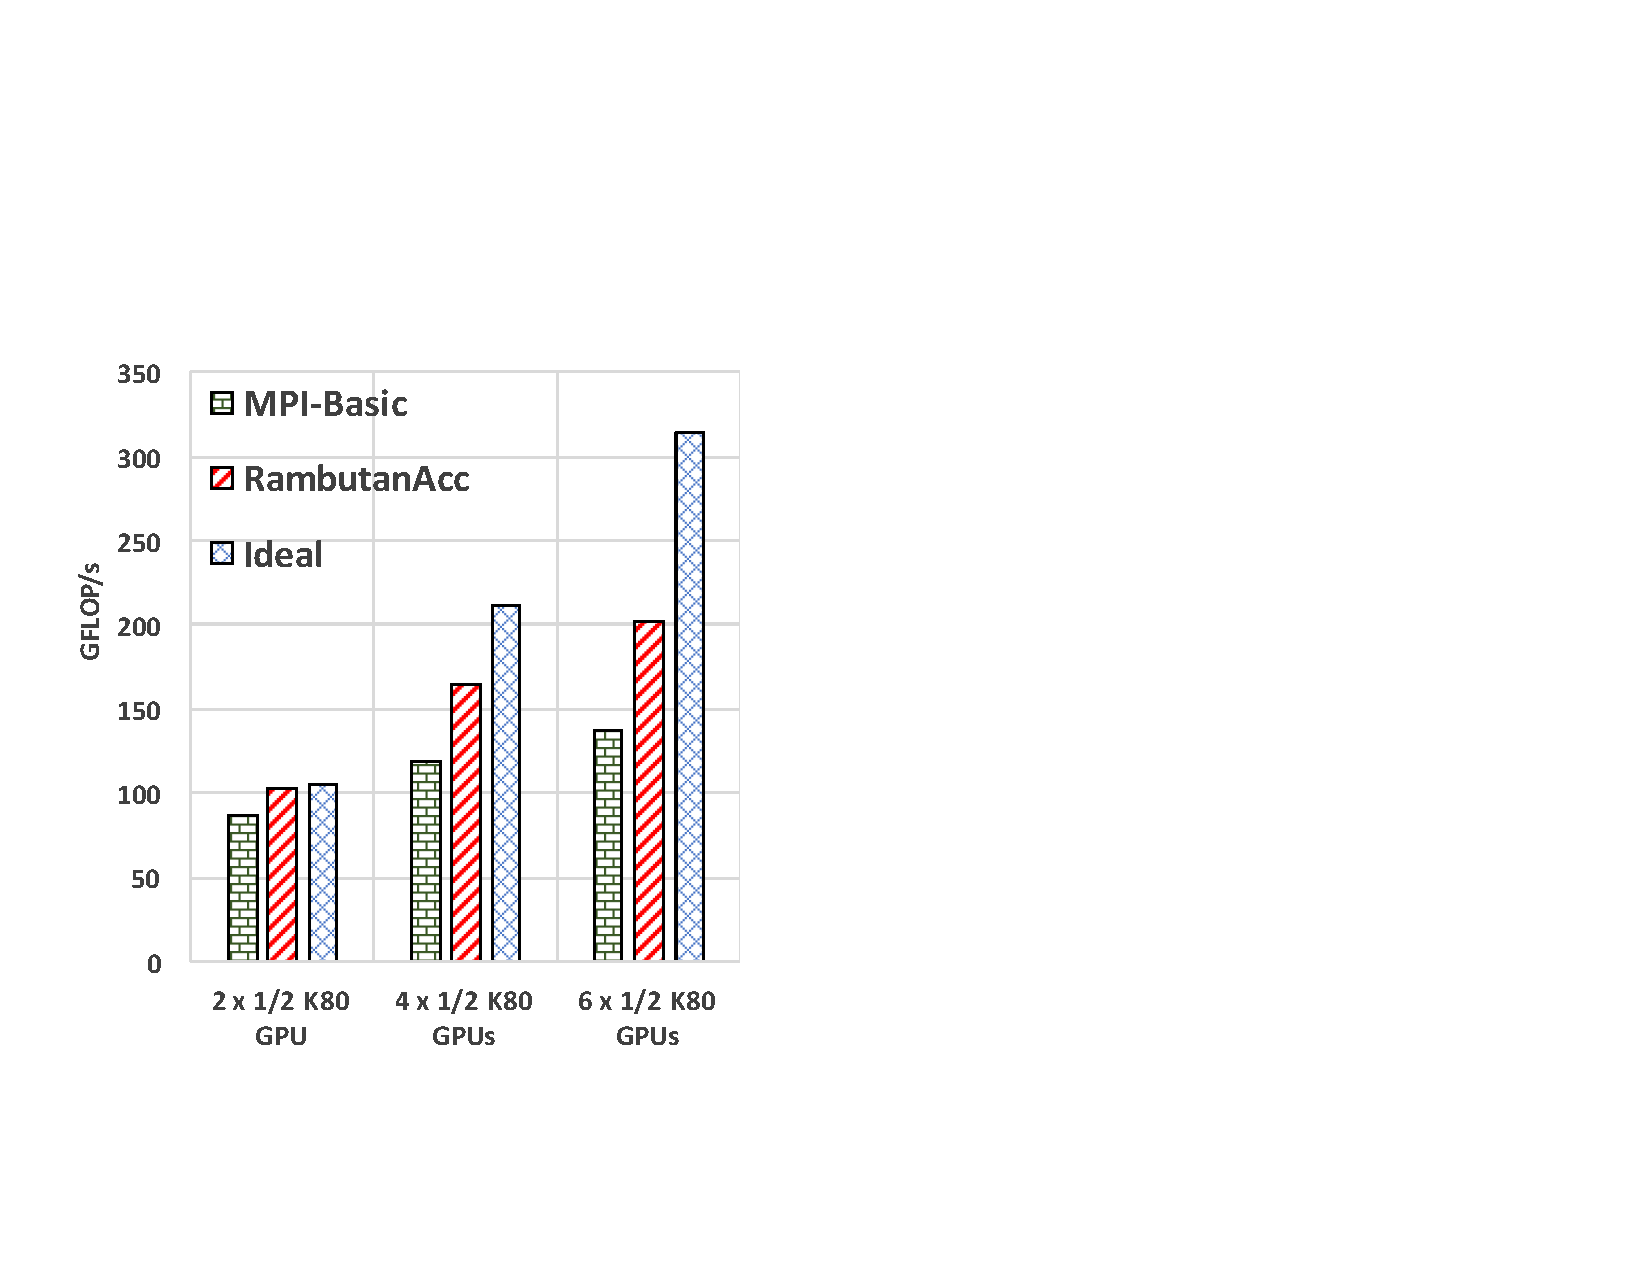
\includegraphics[width=0.49\textwidth]{figures/stencil_tida.pdf}
\caption{Strong scaling study on a single compute node consisting of three K80s (six GPU devices). Problem size $512^3$.}
\label{stencil_onnode}
\end{figure}

\begin{figure*}[htb]
\centering
\begin{subfigure}[b]{0.45\textwidth}
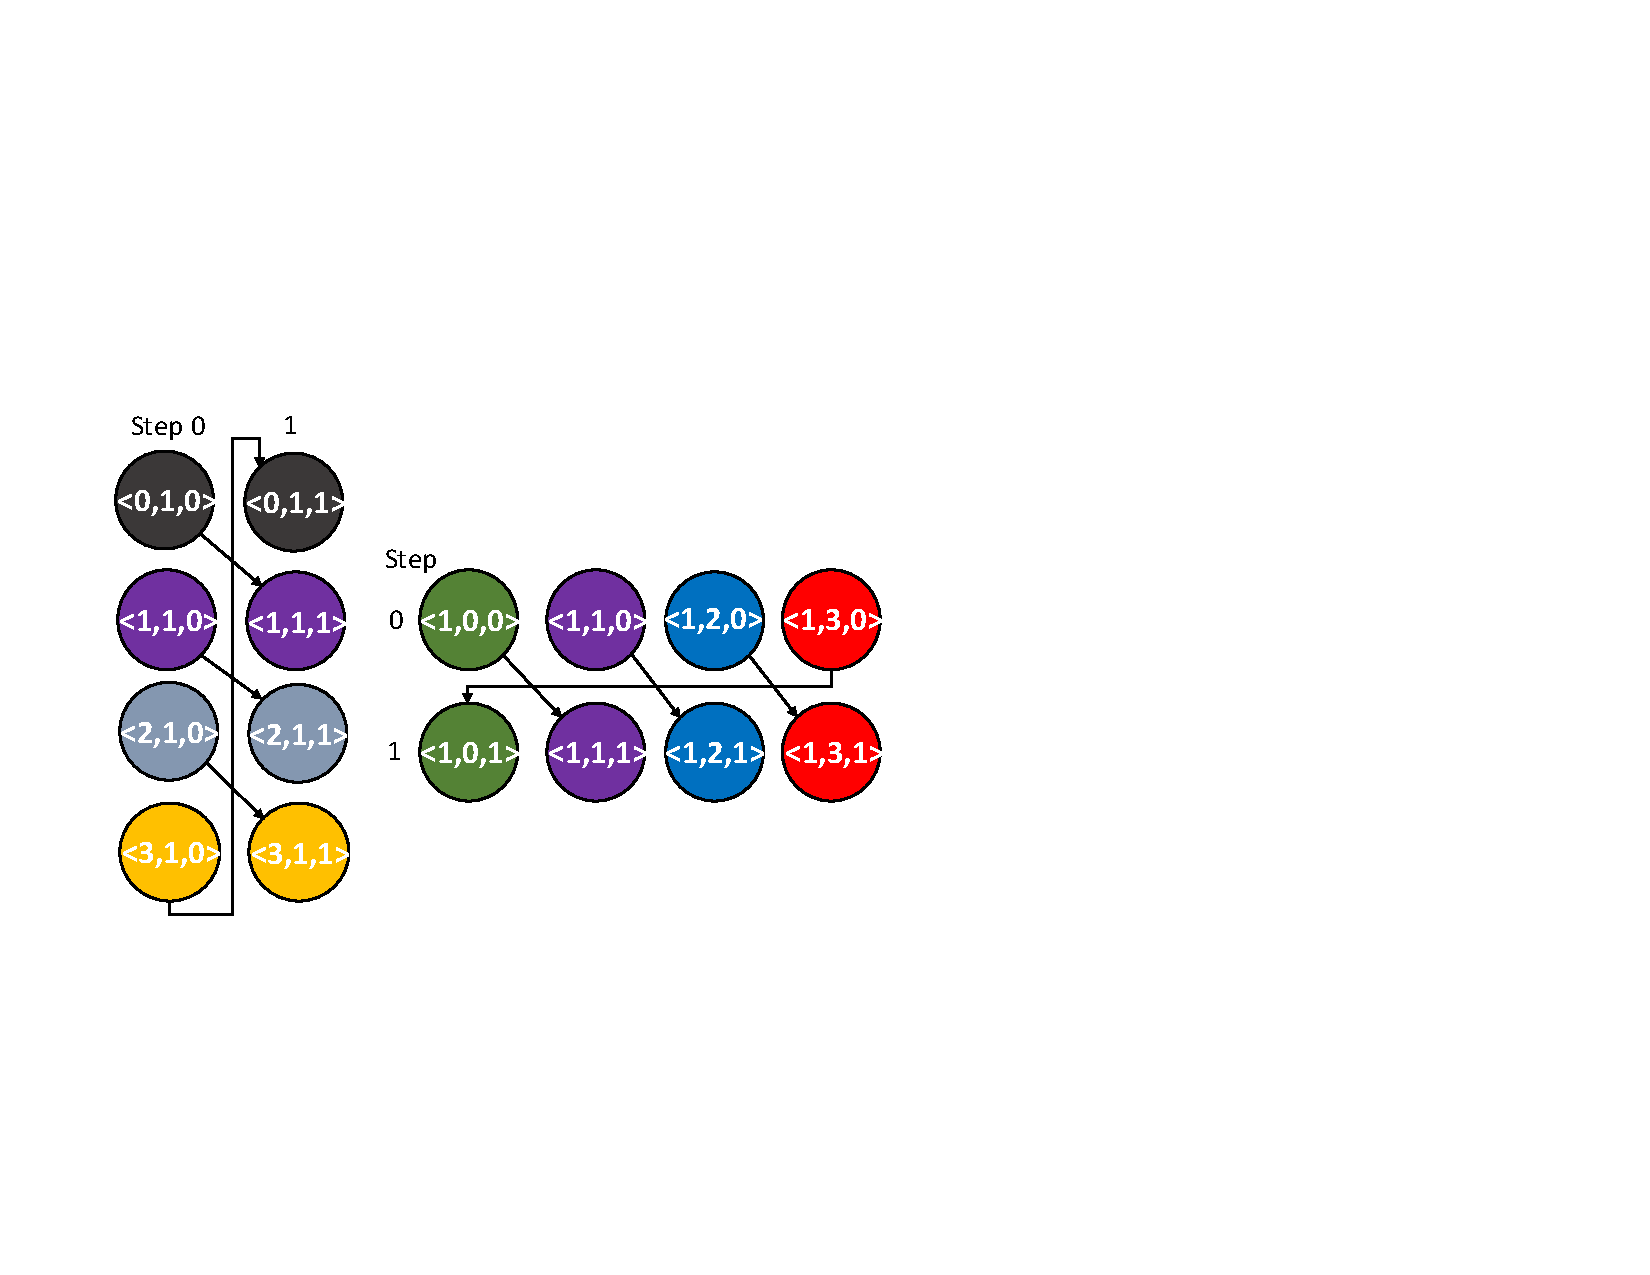
\includegraphics[width=\textwidth]{figures/cannon0.pdf}
\caption{A and B dependencies on each replication layer}
\label{deps}
\end{subfigure}
\begin{subfigure}[b]{0.37\textwidth}
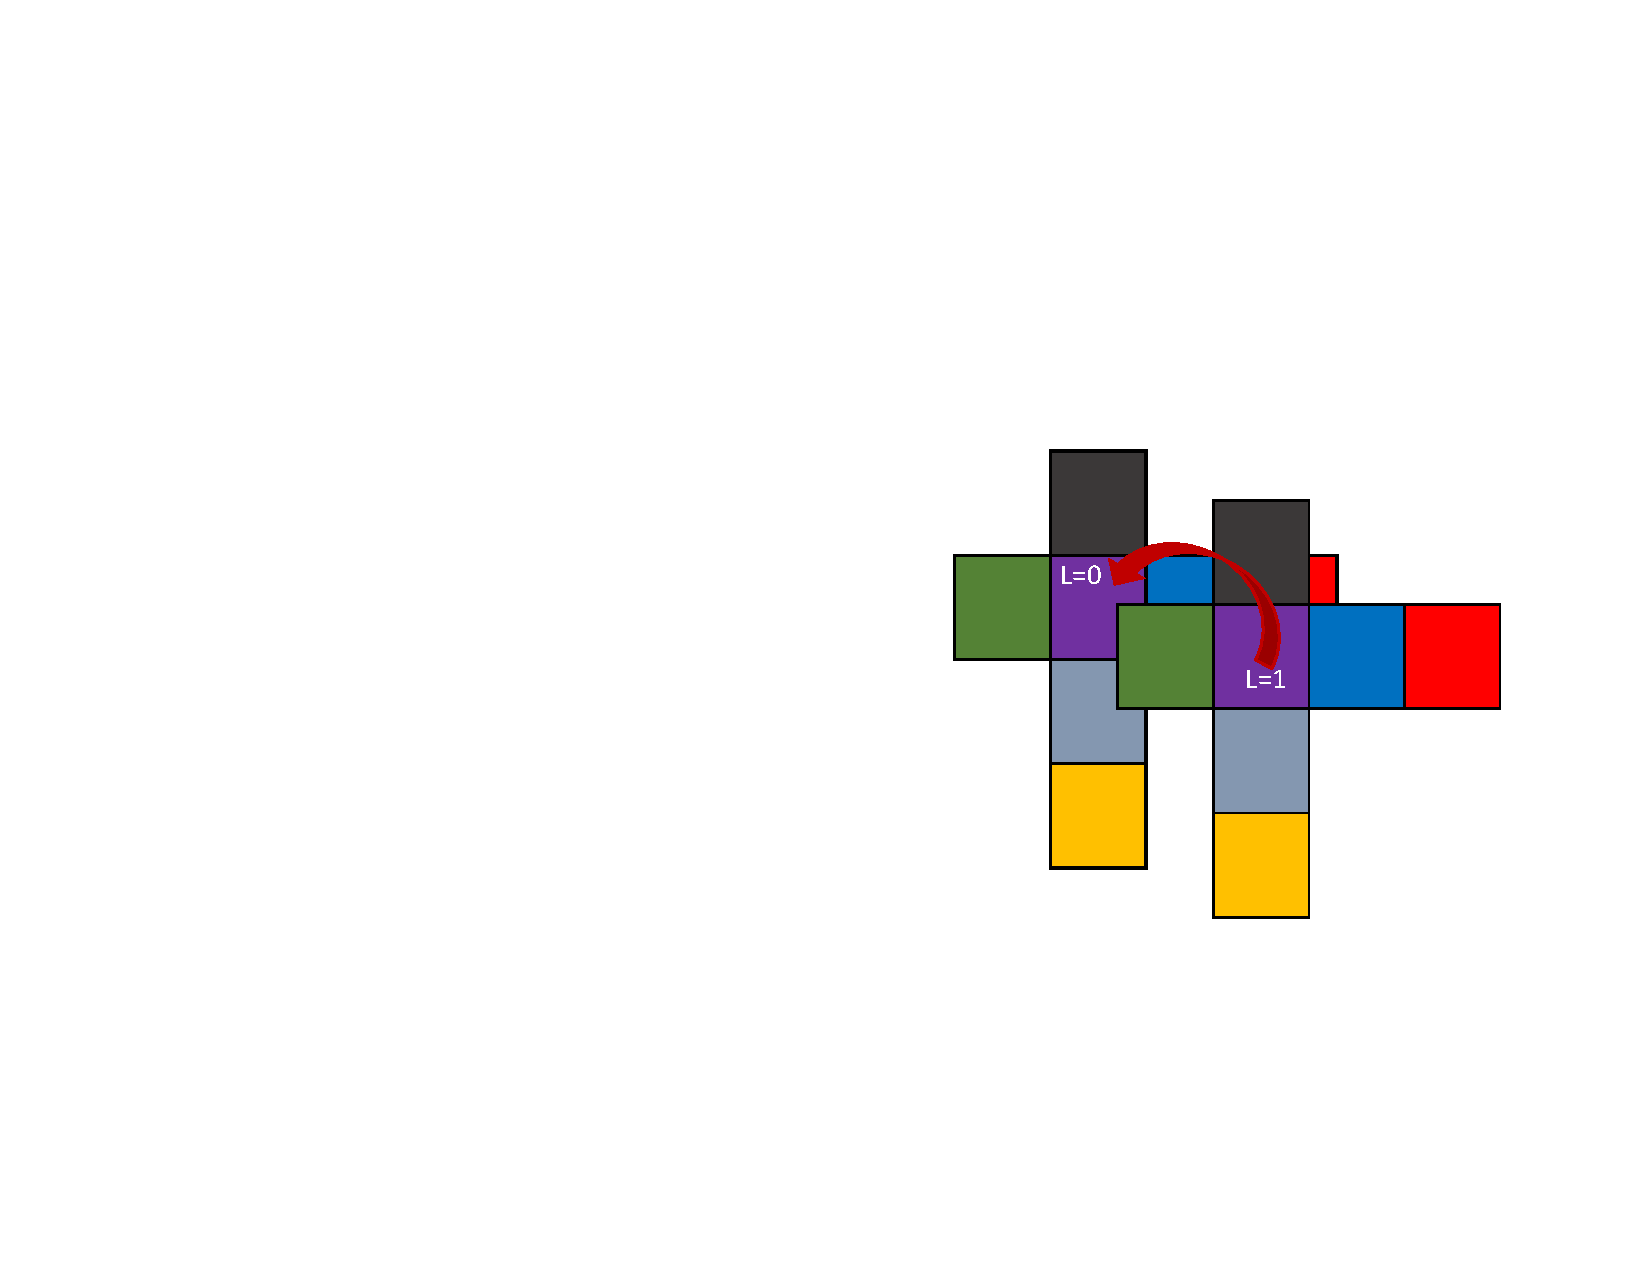
\includegraphics[width=\textwidth]{figures/cannon1.pdf}
\caption{Results are reduced to the original layer}
\label{dataspace}
\end{subfigure}
\caption{Computing $C= \alpha A * B + \beta C$ using the 2.5D Cannon's matrix multiplication algorithm given the input matrices are already replicated and aligned. 
The DAG partitions matrix C and the step space of the algorithm.
Task Id is a triple where the first two numbers represent the coordinates of a C partition and the last is the step number of the algorithm. 
Fig.~\ref{deps} shows two subsets of the graph to illustrate two types of data dependecies required to compute C.}
\label{fig:25DCannon}
\end{figure*}

\subsubsection{2.5D Cannon Matrix Multiply}
Although sparse representations are widely used in practice, dense matrix operations also have a significant share in many scientific and engineering areas.
As a result, we employ a dense matrix multiplication operation $C = \alpha* A * B + \beta C$ to evaluate our runtime.
This is a compute bound application, and the GPU architecture is very well suited for the computation. 
There are many algorithms for the matrix multiply operation, and we use a well-known extension of the standard 2D Cannon's algorithm called {\em Communication Avoiding} or 2.5D Cannon~\cite{25Dcannon}. 
Under the original 2D Cannon's algorithm, the available tasks are organized into a {\em T=PxP} mesh, partitioning each of the three matrices A, B, and C into blocks.
These partitions are first aligned using a skewing operation.
The algorithm then performs P computation steps accumulating the C partition using the rotated A and B partitions.
The communication avoiding algorithm shown in Fig.~\ref{fig:25DCannon} replicates the input matrices by a factor of L using an additional task dimension.
The algorithm broadcasts input data to layers in this dimension to compute the traditional Cannon with T/$\sqrt(L^3)$ steps then reduces the results back to the first layer.



\begin{figure}[htb]
\centering
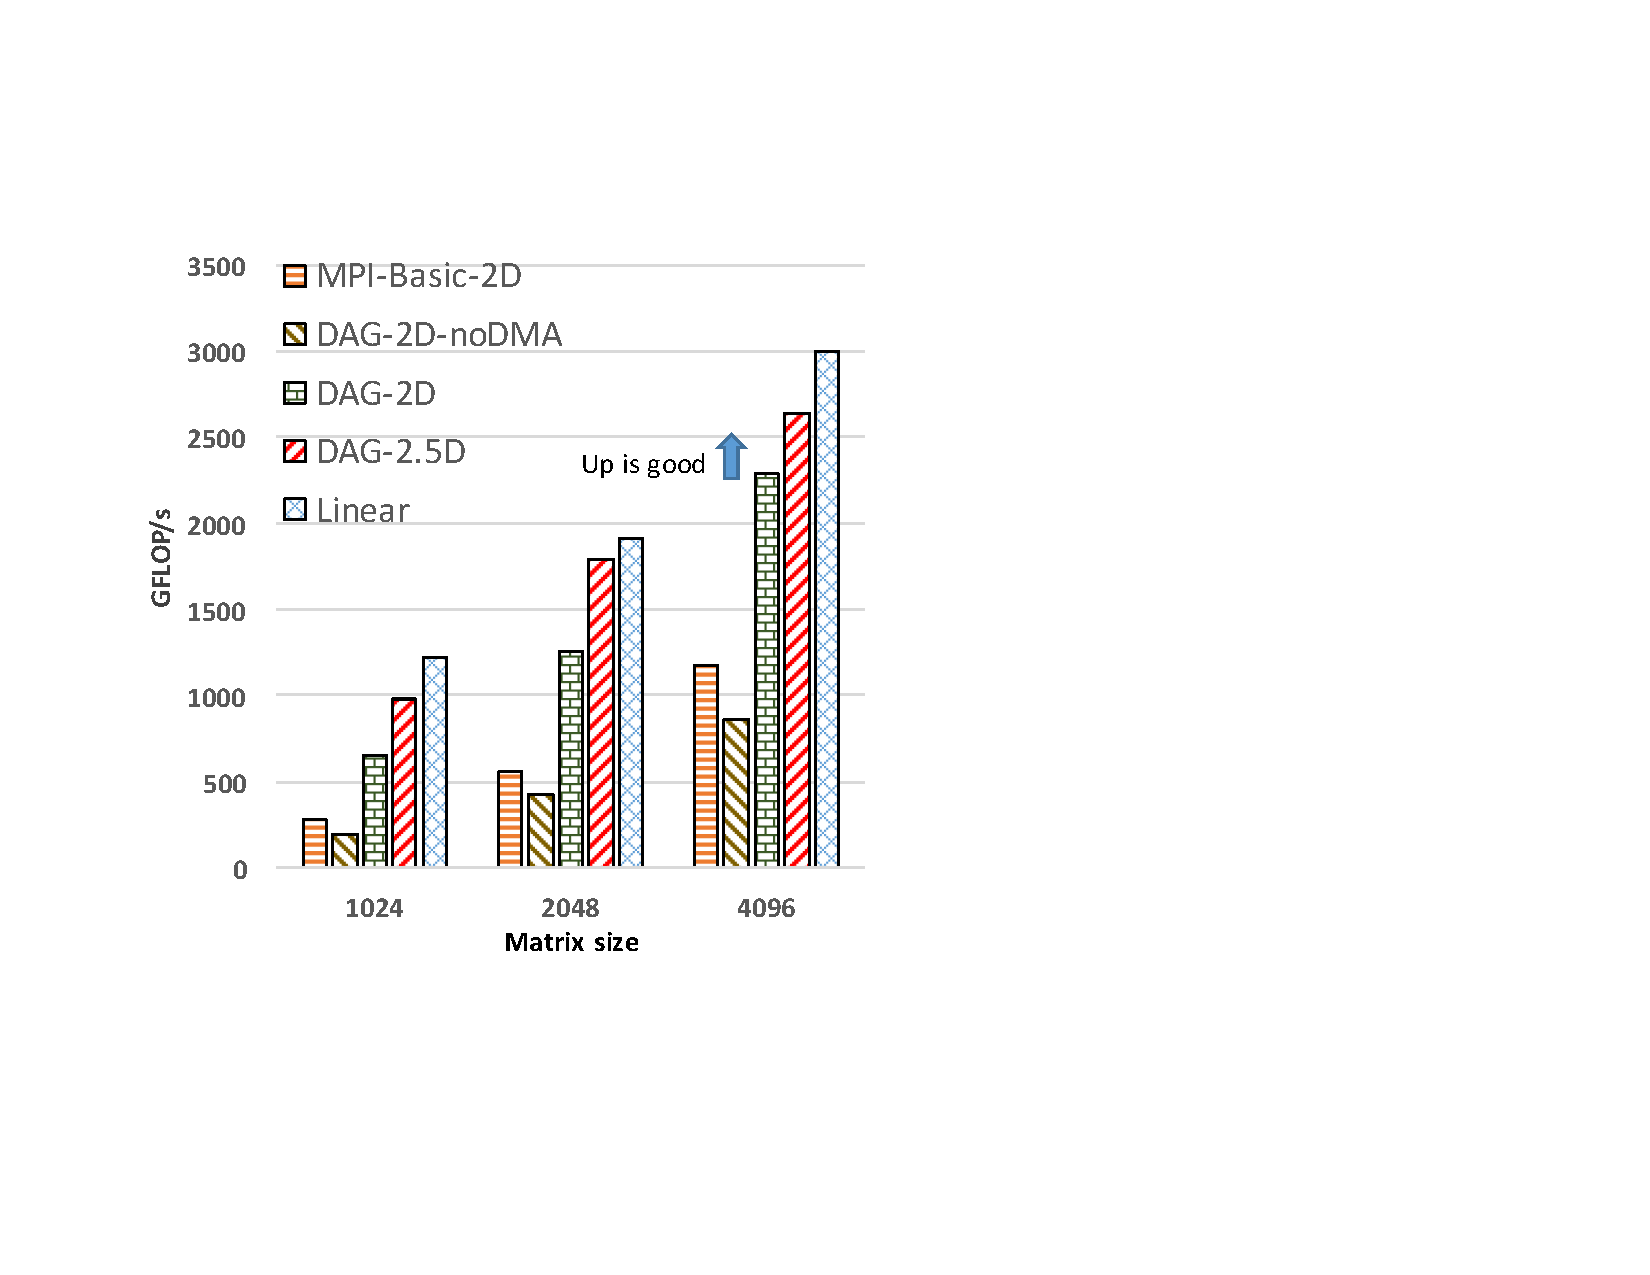
\includegraphics[width=0.49\textwidth]{figures/cannon_tida.pdf}
\caption{2.5 Cannon on two K80s (four GPU devices)}
\label{cannin_onnode}
\end{figure}




\subsection{Scheduling tasks at the cluster level}
%\samW{is this a missing subsection? or is communication hiding supposed to be a subsubsection???}

\subsubsection{Communication hiding}
We now extend the experiment to multiple GPUs.
In this experiment, we evaluate the benefit of hiding the communication overheads among GPUs.
To this end, we configure the runtime in two modes: {\em no overlap} and {\em overlap}.
The former uses blocking CUDA memory copy routines to transfer data between host and GPUs while the latter uses non-blocking variants.
Since the fine-grained scheduler is not compatible with blocking mode (the persistent kernel runs to completion while blocking routines can't proceed until all previously submitted CUDA kernels have completed), we use the coarse-grained scheduling policy for both the blocking and non-blocking modes.

Fig.~\ref{overlap} shows results of three applications under two communication modes.
In this study, we do not replicate the input matrices of the 2.5D Cannon's algorithm because the communication avoiding technique may interfere with the communication overlap.
We will study this interference later in Sec~\ref{subsec:CAvsOlap}.
It can be seen in Fig.~\ref{overlap} that on three applications {\em overlap} always outperforms {\em no overlap}.
In Cholesky, we place data on the host and stream them to GPUs to perform the compute-intensive {\em update} kernel.
Thus, even on one GPU, communication arises.
\footnote{Although we do not show results of 2.5D Cannon and 3D Stencil on one GPU, it's worth noting that computing on one GPU doesn't incur communication cost since we initially place data on the GPU.
As a result, we do not observe performance improvement when running these two applications on only one GPU.}
On multiple GPUs, we realize notable performance improvement via overlapping communcation with computation.
The overall time reduction is 10\% more or less.
For Stencil, however, we see a higher speedup (up to 1.85$\times$) due to the following reason.
At a small scale 1D decomposition works best since it does not require the costly packing and unpacking operations.
However, with a 1D decomposition scheme the amount of communication does not decrease as the number of GPUs increases.
Thus, the more GPUs the higher communication relative to computation, resulting in a better improvement due to overlap.
Unlike 3D Stencil, experiments on the other two applications use a 2D decomposition scheme.
Thus, the communication over computation ratio does not change much as the number of GPU increases.

\begin{figure*}[htb]
\centering
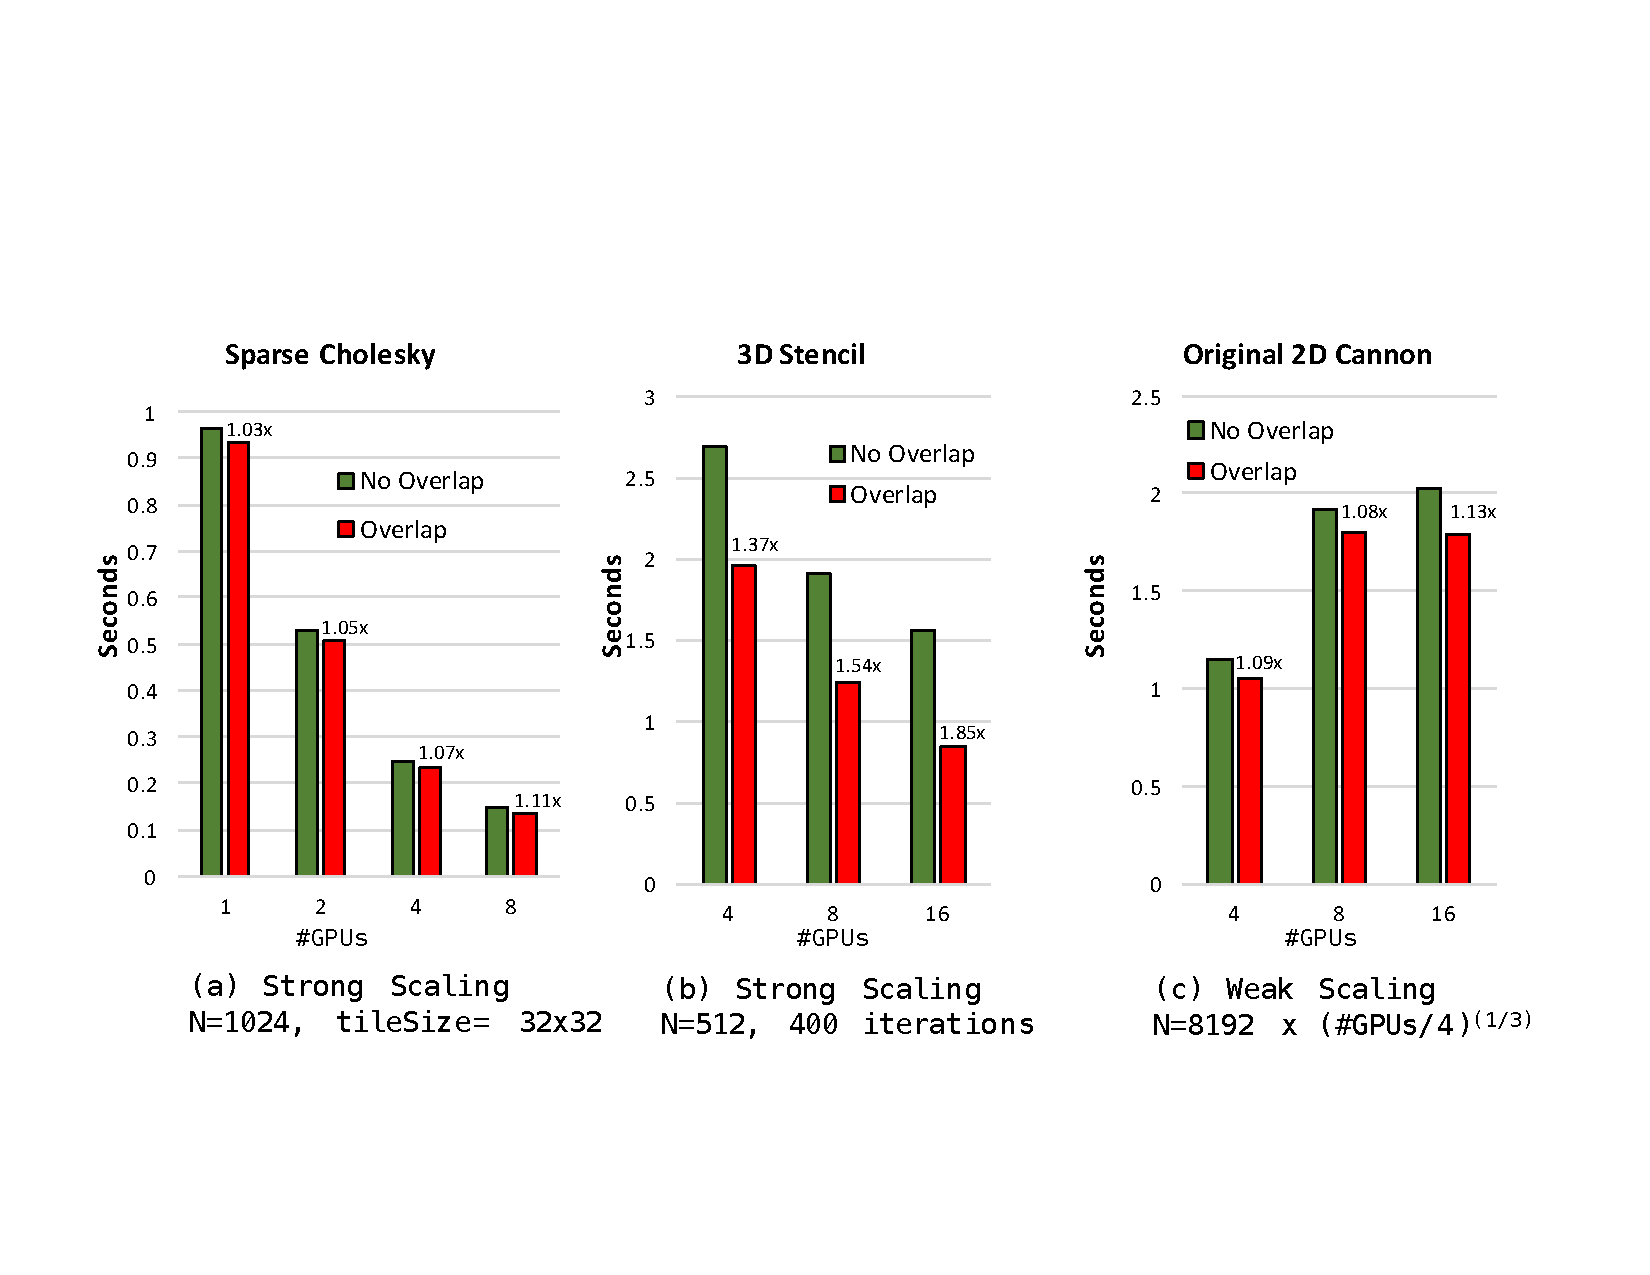
\includegraphics[width=0.9\textwidth]{figures/overlap.pdf}
\caption{Hiding communication automatically via overlap}
\label{overlap}
\end{figure*}

\begin{figure}[htb]
\centering
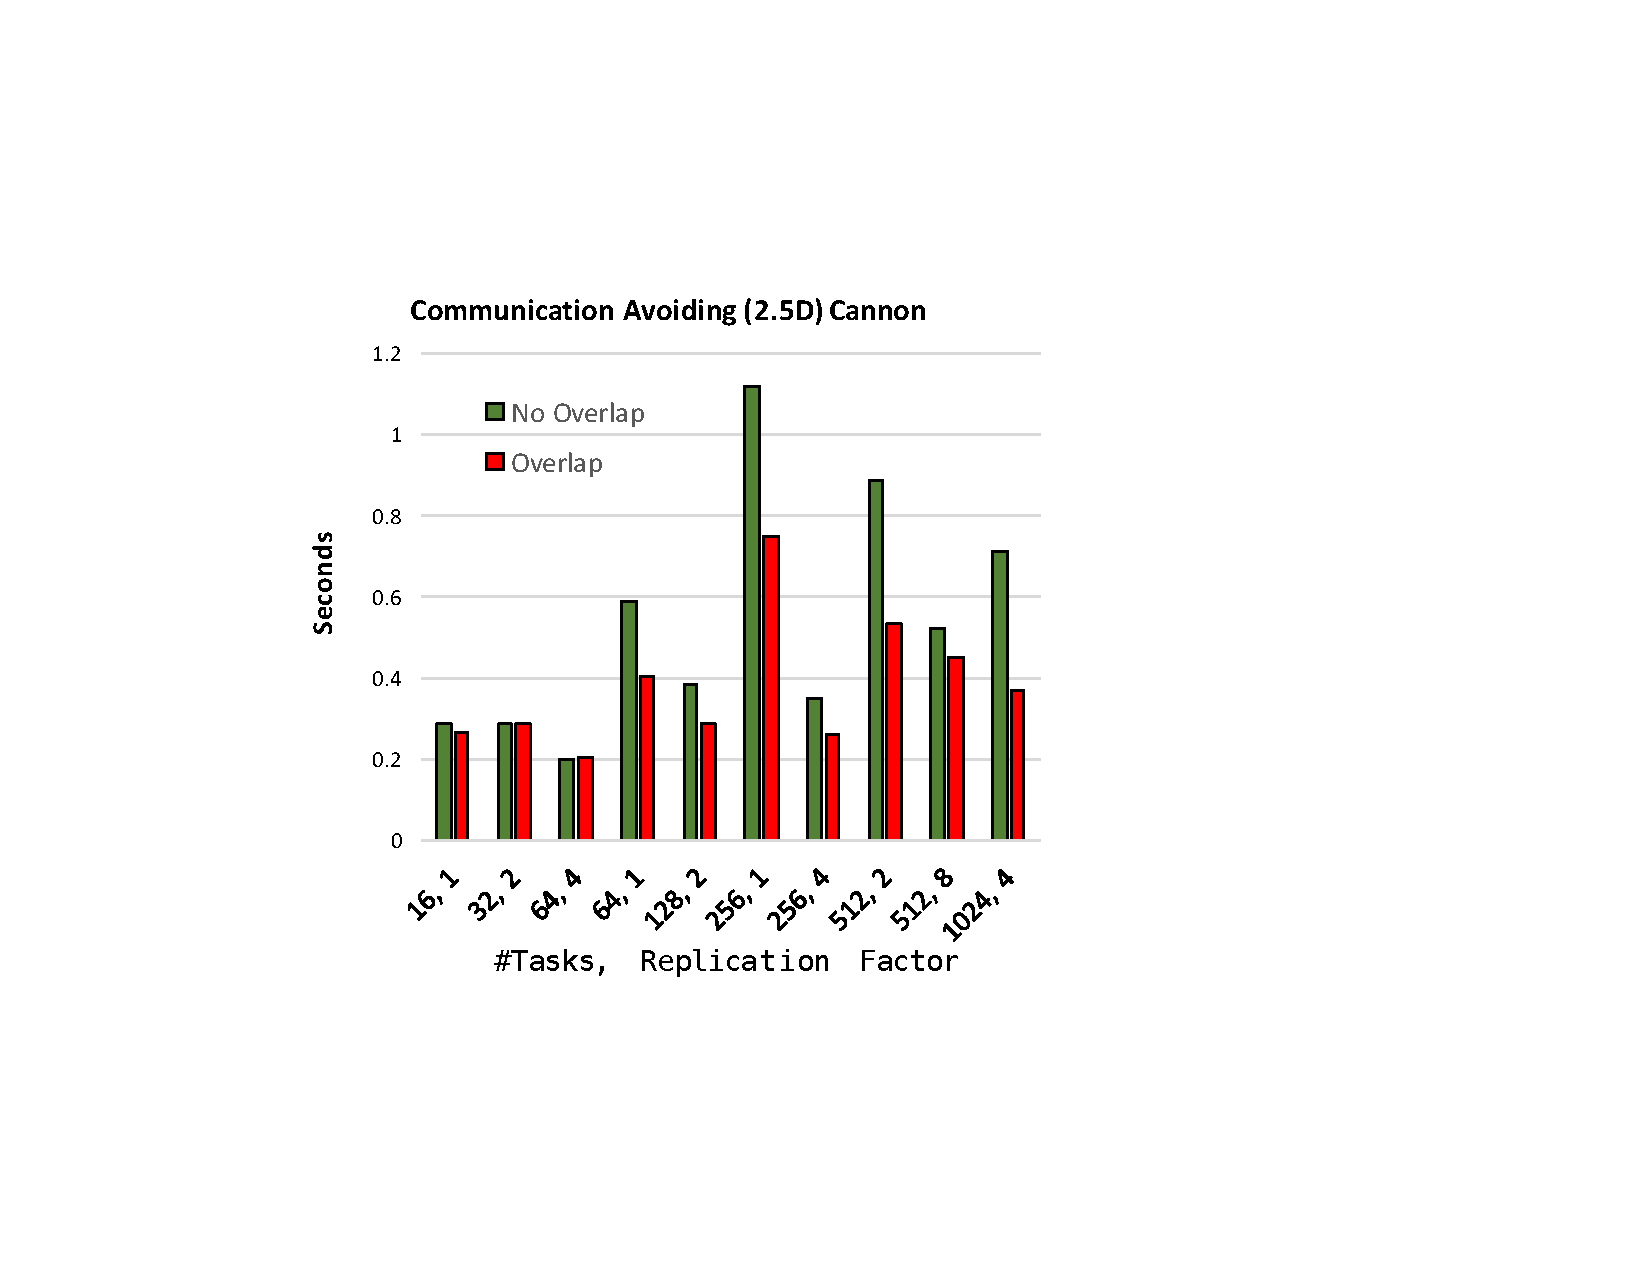
\includegraphics[width=0.49\textwidth]{figures/CA_4096.pdf}
\caption{2.5D Cannon on 16 GPUs using small matrices (N=4096). The communication avoiding technique results in many task configurations. For good configurations (e.g. \{64, 4\}), there is not much room for the communication overlap. However, for poor configurations (e.g. \{1024, 4\}) the overlap technique does a good job in further increasing the performance}
\label{CA_4096}
\end{figure}

\subsubsection{Interference between communication avoiding and hiding}
\label{subsec:CAvsOlap}
Now let's study the behavior of {\em overlap} when the communication avoiding technique is enabled.
Fig.~\ref{CA_4096} shows the run time of the 2.5D Cannon program when performing matrix multiplication on 16 GPUs.
We can see that replicating matrices substantially reduces the run time.
Notable examples are  \{64, 4\} compared to \{64, 1\} and \{256, 4\} compared to \{256, 1\}.
If most of the data communication can be avoided, there is not much left to hide.
However, the number of these optimal replication configurations is very small compared to the combination of task and replication spaces.
As a result, the programmer may need to brute force many potential configurations to find the best one.
This requirement is costly and time consuming.
Luckily the overlapping technique can work with communication avoiding within the same application.
Thus, if the programmer does not pick the best replication configuration, he/she can rely on the communication overlap to realize comparable performance.
For example, the {\em overlap} performance on configurations \{128, 2\}, \{256, 4\}, or the most wanted \{64, 1\} is  acceptable. 
We can see that there are many of such configurations, allowing the programmer to guess one easily.



\section{Related work}
\label{sec:related}
The benefit of using a data-driven execution model on traditional multi-core processors has been recognized by the HPC community for years, e.g. Cilk/Cilk++~\cite{cilk,BlumofeJoKu95}, Charm/Charm++~\cite{charm++}, Tarragon/Bamboo~\cite{cicotti11:dissertation,bamboo, bamboo-LU, bambooThesis}, DPLASMA\cite{dplasma,Bosilca:2012:DAGuE}, OMPSs~\cite{ompss,nexus}, and Habanero-C MPI~\cite{Chatterjee:2013:HCMPI}.
However, the question of whether a task dependency graph program with many fine-grained tasks can run efficiently on an accelerator (e.g. GPU) has not yet been thoroughly answered.
As a result, many current runtimes for GPUs schedule each single task on the whole GPU (e.g. Legion~\cite{legion} and CNC-HC~\cite{cnc-hc}).
As the number of cores per accelerator increases quickly, this limitation puts the programmer under the pressure of optimizing their kernels so they can scale linearly as the accelerator architecture evolves.

Recently more research has been focusing on launching a CUDA kernel on a portion of the GPU.
In~\cite{fillNRetreat}, Wu et al. presented a technique called {\em fill and retreat}, which allows a CUDA kernel to run on a group of selected SMs.
With this technique the programmer can efficiently bundle multiple CUDA kernels to run on a single GPU at a time.
Abdelfattah et al. also used a similar technique to batch small CUDA kernels in a cholesky factorization program in order to improve the throughput~\cite{batchedCholesky}.
Our solution relies on a task scheduler to factor the scheduling policy out of the application program.
As a result, the programmer can take the benefit of fine-grained scheduling at a very small amount of programming cost.

Multi-GPU programming is also an important support because the memory capacity of each individual GPU is very limited.
There are MPI implementations that provide this support, e.g. MPI-ACC~\cite{mpiacc, mpiacc1} and Mvapich~\cite{mvapich2gpu}.
However, with these tools the programmer has to explicitly move data.
RambutanAcc provides a dataflow programming model that supports distributed-memory architectures, allowing the runtime to move data across memory address spaces transparently.
In addition, the data movement is non-blocking and independent of computations, overlapping communication with computation.

{\em RambutanAcc} is a general-purpose runtime system and programming model.
Thus, it supports a wide range of applications, as opposed to other domain-specific runtimes such as MAGMA~\cite{MAGMA}, Physics~\cite{physics}, and Patus~\cite{patus}.


\section{Conclusion}
\label{sec:conclusion}
We have presented {\em RambutanAcc}, a programming model and runtime system for accelerator-based clusters.
Experimental results on 3 benchmarks using up 16 K80 GPUs show that with {\em RambutanAcc} the programmer can realize better performance.
The performance improvement comes from increasing throughput of processing fine-grained tasks on each individual GPUs and/or hiding communication overheads among GPUs.
{\em RambutanAcc} offers a simple interface so the programmer can achieve these benefits without the needs of redesigning the algorithm and aggressively restructuring the source code as the system architecture evolves.
We deem that our paper not only has impact on application development, but it can also initiate further research on HPC libraries such as developing and tuning cuSPARSE routines for running on the same GPUs. 


\section*{Acknowledgments}
% DOUBLE BLIND
%This material is based upon work supported by the Advanced Scientific Computing Research Program in the U.S. Department of Energy, Office of Science, under  Award Number DE-AC02-05CH11231.
%RambutanAcc and application codes were developed on TiDA, a workstation housed at LBNL, with GPUs provided by NVIDIA.
%Experiments were conducted on Comet at SDSC.
%We would like to thank Paul Hargrove for his great help on GASNet.
%We also thank Yifeng Cui for time allocations on the Comet system.
%Tan Nguyen was a fellow of the Vietnam Education Foundation while conducting this research.

%\input{artifact}

\bibliographystyle{ACM-Reference-Format}
\bibliography{ref} 


\end{document}
